This thesis project has involved the implementation and evaluation
of many different components required to create an end-to-end wheelchair
navigation assistance system.

\subsection{Evaluation of machine learning models on preliminary dataset}
%include speed
The YOLOv5, DeepLabv3, and Hybridnets models were tested on the preliminary
video-only Curtin driving dataset. As this dataset is unlabelled, the
models were evaluated in terms of speed and potential usage, rather than accuracy.

A frame of YOLOv5 evaluated on the preliminary dataset can be seen in \cref{fig:yolov5s}.
This model identifies vehicles and pedestrians with high accuracy, with the confidence in
a prediction decreasing as the object moves further away from the camera.

A frame of DeepLabv3 evaluated on the preliminary dataset can be seen in \cref{fig:deeplab}.
DeepLabv3 identifies pedestrians with a high level of accuracy. However, the vehicles in the
image are not accurately segmented. This is likely due to the lower occurrence of vehicles
in the MS COCO dataset, which was used to train the model.
To repurpose this model for the task of drivable area segmentation,
it would have to be retrained on a labelled driving dataset such as BDD100K or Cityscapes.

\begin{figure}[b]
    \centering
    \begin{minipage}[b]{.45\textwidth}
        \centering
        \captionsetup{width=.8\textwidth}
        \includegraphics[width=\linewidth]{images/yolov5s_cropped.png}
        \captionof{figure}{YOLOv5s evaluated on the Curtin dataset}
        \label{fig:yolov5s}
    \end{minipage}%
    \quad
    \begin{minipage}[b]{.45\textwidth}
        \centering
        \captionsetup{width=.8\textwidth}
        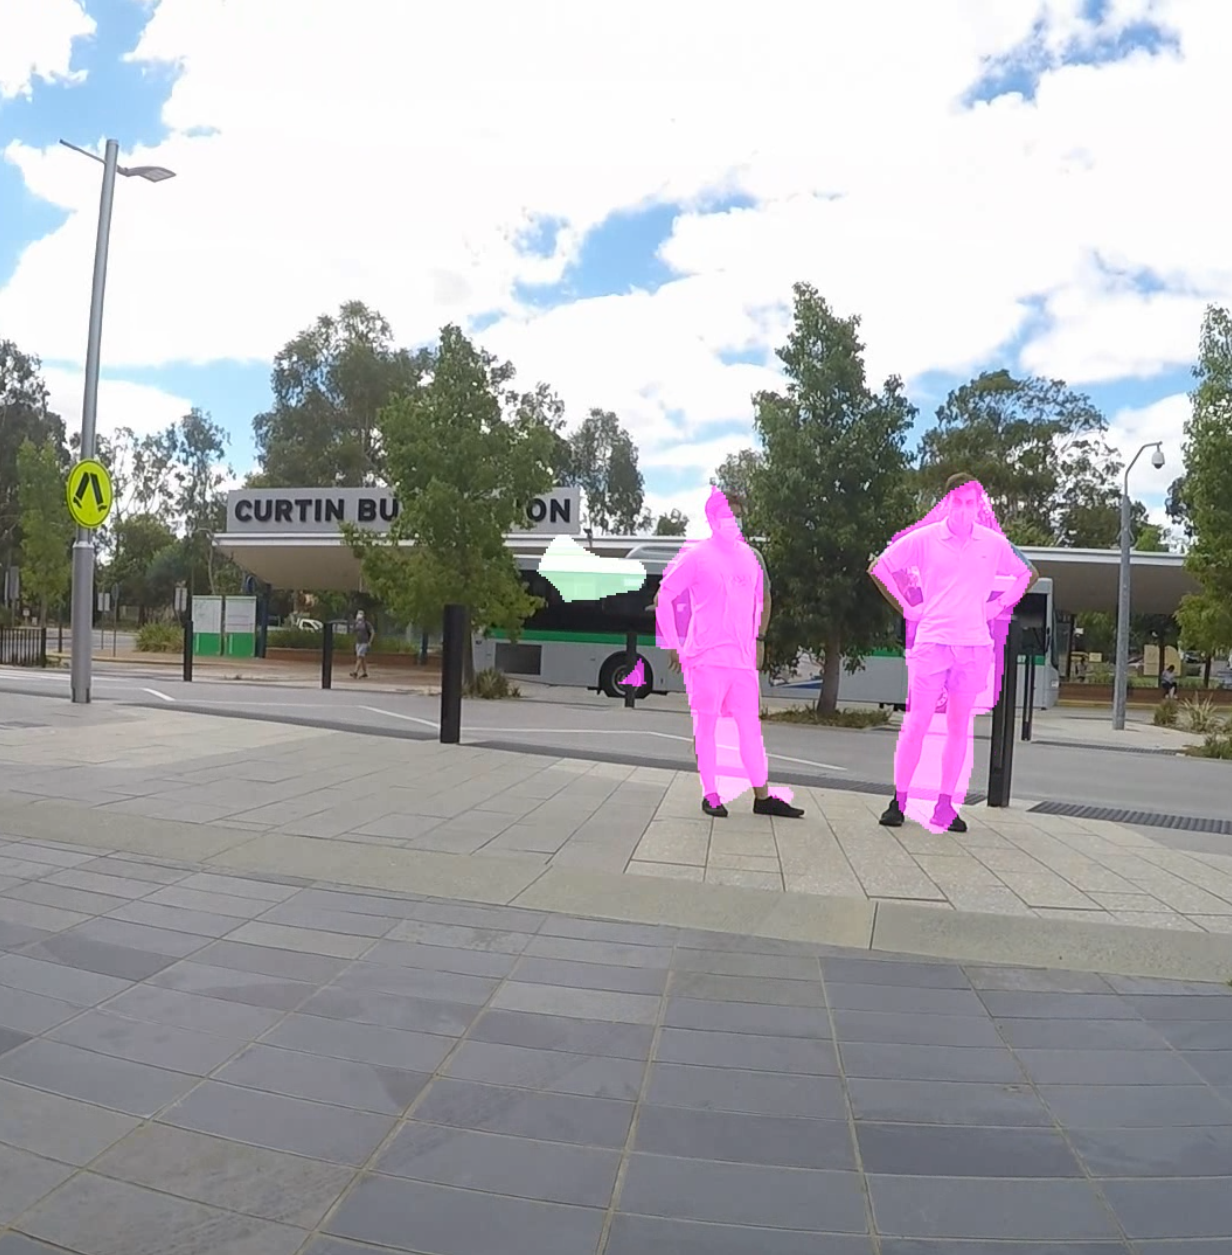
\includegraphics[width=\linewidth]{images/deeplab_cropped.png}
        \captionof{figure}{DeepLabv3 evaluated on the Curtin dataset}
        \label{fig:deeplab}
    \end{minipage}
\end{figure}

An example of Hybridnets drivable area segmentation can be seen in \cref{fig:hybridnets}.
This model accurately detects drivable areas outdoors when a path is uniform, however
has more difficulty identifying a drivable path for non-uniform surfaces such as paved brick.
Hybridnets can also struggle to identify drivable paths indoors in some circumstances.
This is likely due to problems with domain adaptation, as the Hybridnets model was trained on the
BDD100K dataset which primarily consists of bitumen roads.
Hybridnets does not identify drivable area consistently when indoors
but does work well in some cases.

\begin{figure}[b]
    \centering
    \begin{subfigure}{.48\textwidth}
        \centering
        \includegraphics[width=\linewidth]{images/hybridnets_outdoor.png}
        \caption{Outdoors}
    \end{subfigure}
    \quad
    \begin{subfigure}{.47\textwidth}
        \centering
        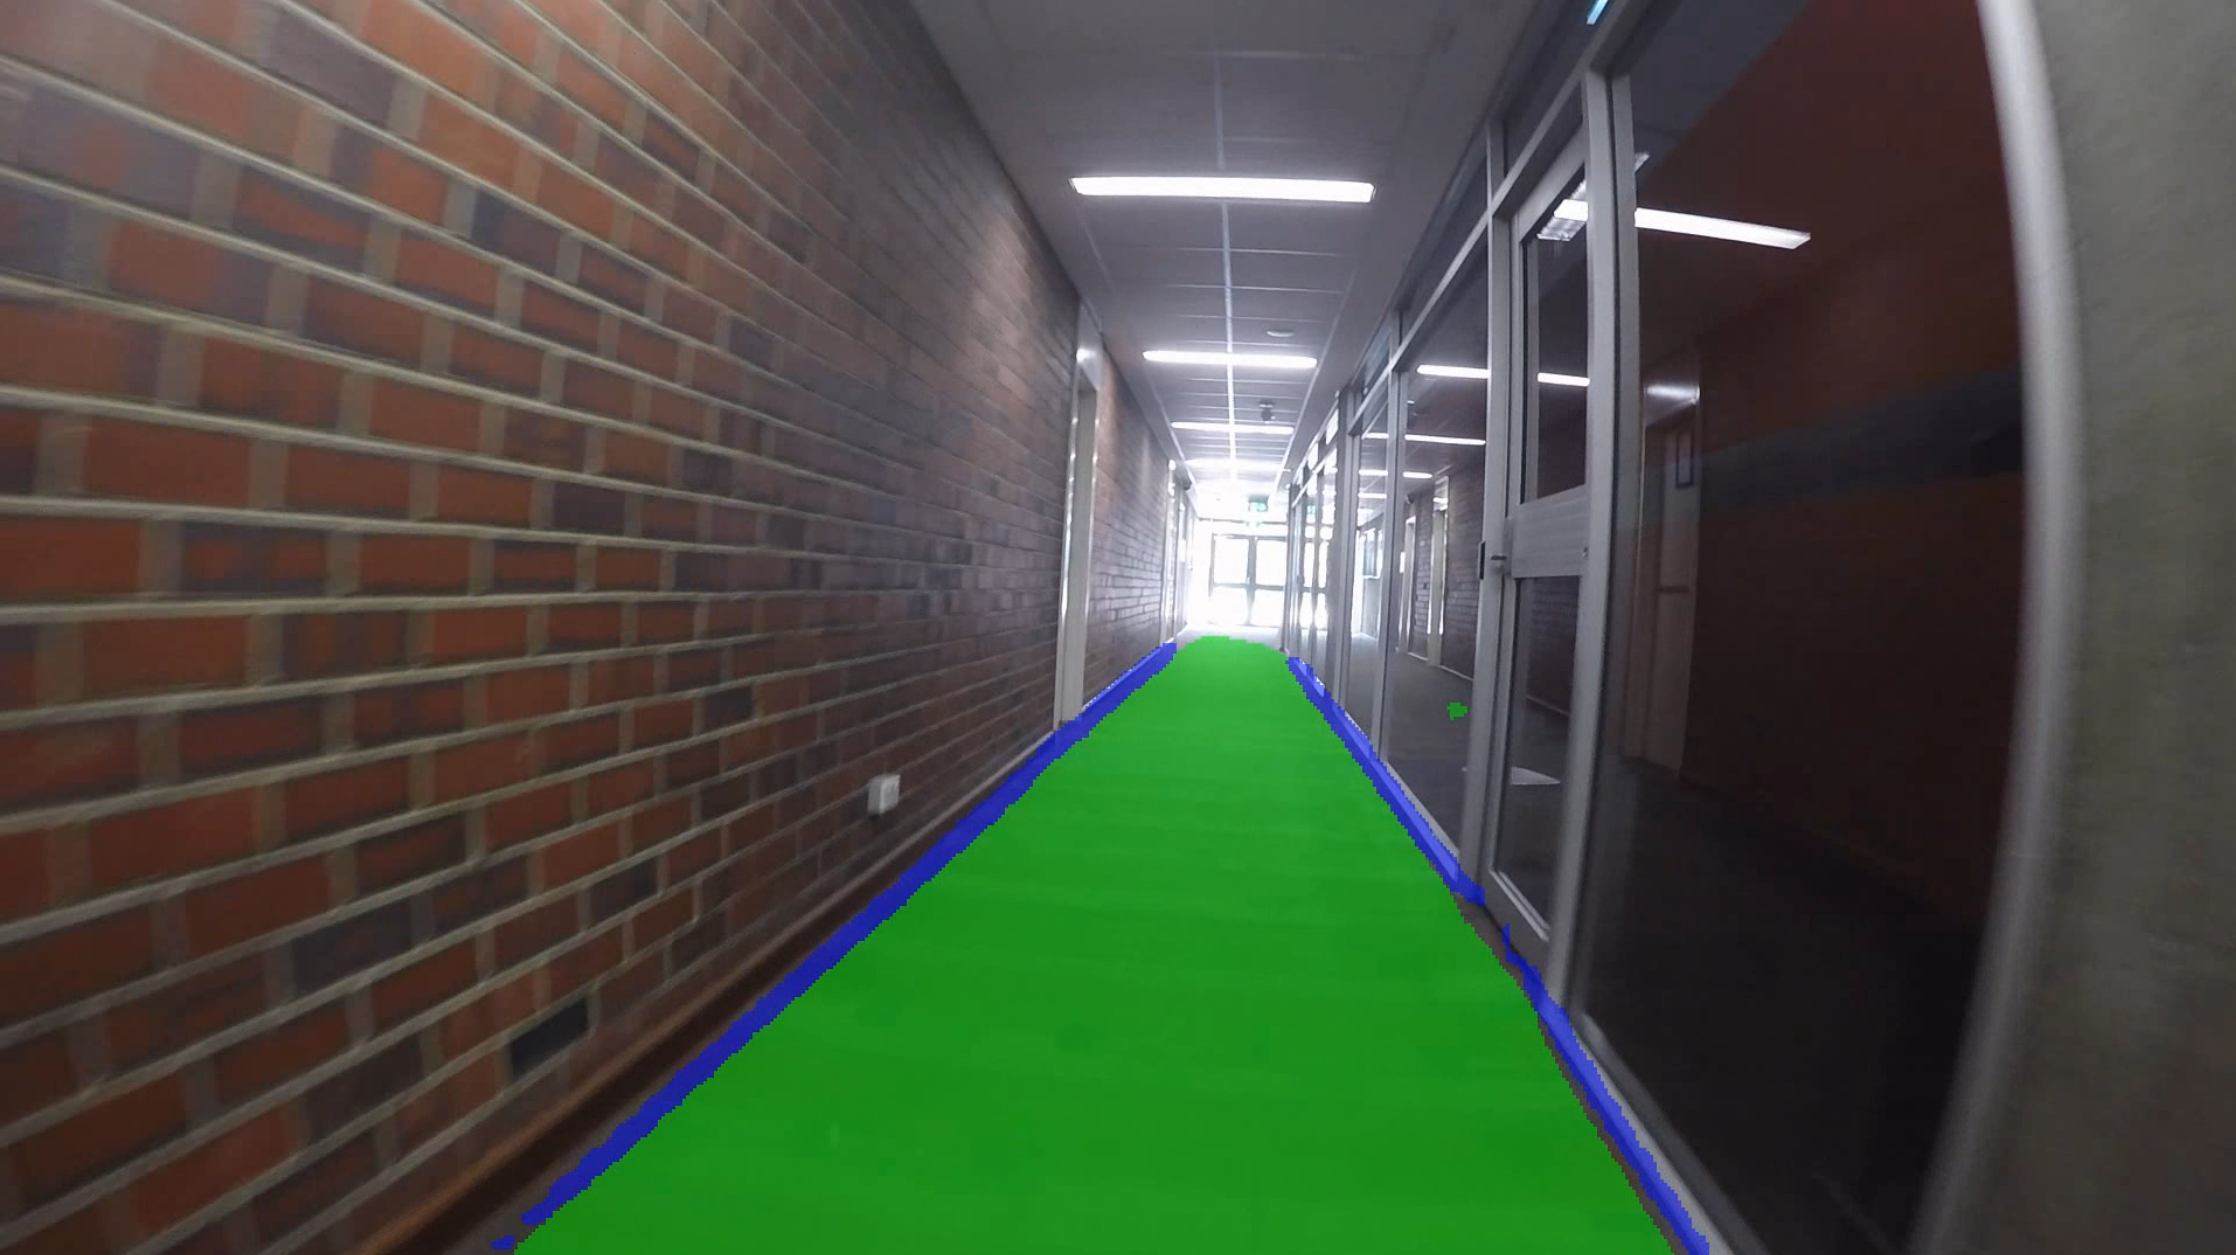
\includegraphics[width=\linewidth]{images/hybridnets_indoor.png}
        \caption{Indoors}
    \end{subfigure}
    \caption{Hybridnet drivable area segmentation evaluated on the Curtin dataset}
    \label{fig:hybridnets}
\end{figure}

The performance of each model (in frames per second) is given in \cref{table:model_fps}.
This performance was evaluated using a laptop with an RTX 3080 graphics card and AMD Ryzen 9 6900HX processor.
Note that Hybridnets is CPU limited, and could likely be optimized further by modifying postprocessing and video decoding methods.
Additionally,
Hybridnets runs both object detection and image segmentation using the same model.
YOLOv5 runs in real-time on our 24fps dataset, and can likely reach much higher speeds.

\begin{table}[H]
    \centering
    \begin{tabular}{c c c}
    Model Name & FPS & Notes \\
    YOLOv5 & Real-time & (Frame-rate of dataset was 24fps) \\
    DeepLabv3 & 21 & - \\
    Hybridnets & 10 & CPU limited (can likely be optimized) \\
    \end{tabular}
    \caption{Performance comparison of ML models}
    \label{table:model_fps}
\end{table}

\pagebreak
\subsection{Hybridnets drivable area segmentation}
% do this first
Evaluating the pretrained Hybridnets model on the BDD100K validation dataset gives a mIoU
of 0.857. When the same model is evaluated against the Cityscapes dataset,
the model achieves a mIoU of 0.266. This difference is due to the methodology behind
the labelling of these datasets: Cityscapes labels all road surfaces as 'road',
whereas BDD100K only labels the current lane as 'drivable'. This can be seen in \cref{fig:dataset_comparison}.

The recall for road detection on the Cityscapes dataset is 30.6\%, whereas the recall for
sidewalk detection is only 1.52\%. Sidewalks are a much smaller segmentation target than
roads in this dataset; refer to \cref{table:pretrained_confusion_matrix} for the
confusion matrix after evaluation.

\begin{table}[H]
    \centering
    \begin{tabular}{|c|c|c|c|}
    \hline
    & None & Road & Sidewalk \\
    \hline
    Non-drivable & 81.0\% & 11.4\% & 2.33\% \\
    \hline
    Drivable & 0.197\% & 5.03\% & 0.036\% \\
    \hline
    \end{tabular}
    \caption{Confusion matrix of Hybridnets model on Cityscapes dataset (before training)}
    \label{table:pretrained_confusion_matrix}
\end{table}

\begin{figure}[b]
    % 16:6 width ratio
    % 0.64, 0.24
    \centering
    \begin{subfigure}{.45\textwidth}
        \centering
        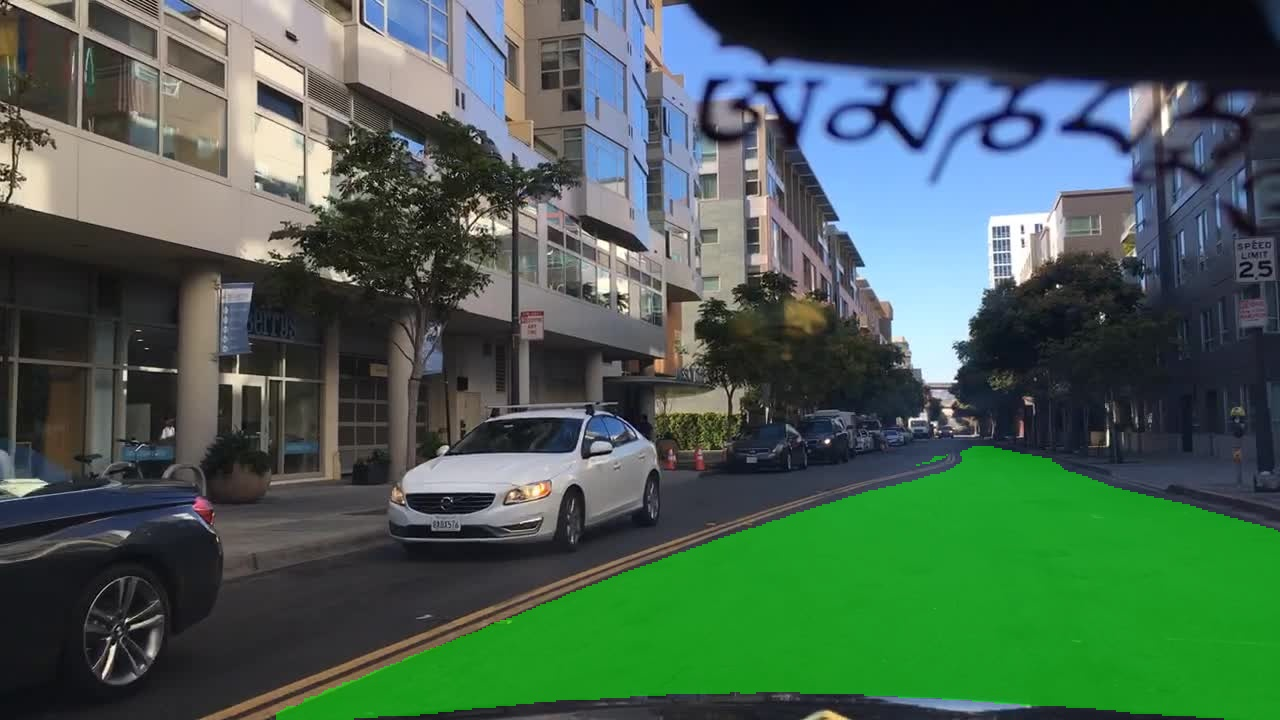
\includegraphics[width=\linewidth]{images/bdd100k.jpg}
        \caption{BDD100K}
    \end{subfigure}
    \quad
    \begin{subfigure}{.45\textwidth}
        \centering
        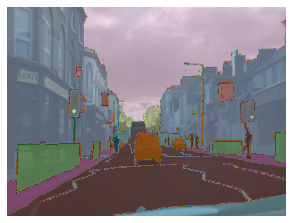
\includegraphics[width=\linewidth]{images/cityscapes.png}
        \caption{Cityscapes}
    \end{subfigure}
    \caption{BDD100K drivable area compared with Cityscapes road segmentation}
    \label{fig:dataset_comparison}
\end{figure}

The model generalises to the new dataset very quickly during training,
as seen in \cref{fig:hybridnet_training_curve}. The validation accuracy vastly
increases after the first epoch, with not much change after that point
apart from a further drop in training loss (which can indicate overfitting).

After epoch 1, the mIoU is 87.5\% (a 56.9\% improvement), with a
road detection recall of 96.2\% and sidewalk detection recall of
68.2\%. As seen in the training curve, the sidewalk detection recall
varies epoch to epoch, with a variance of 4.2\%. This higher variance is
due to the lower occurance of sidewalks in the dataset (compared to roads).

\Cref{fig:compare_trained_hybridnets} shows an example of the retrained Hybridnets model
(epoch 1) compared to the pre-trained model, evaluated on the Curtin driving dataset.
The new model identifies the paved drivable area further away from
the wheelchair but struggles to identify the drivable area directly in front of the wheelchair.
This is still an improvement compared to the pre-trained model, which does not identify any drivable
area at all.

The retrained model (Cityscapes) produces a much noisier output than the pre-trained model (BDD100K).
This could be due to the structure of the Cityscapes dataset - as pedestrian paths are often
separated from the road by verges, the drivable area is more likely to be disconnected.
This is another domain adaptation problem - although the model may identify pedestrian
pathways easily from the viewpoint of a road, it can struggle with identifying these
same pathways from a wheelchair user's perspective. This would also explain the
retrained model struggling to identify the paved drivable area directly in front of the wheelchair.

\begin{figure}[H]
    \centering
    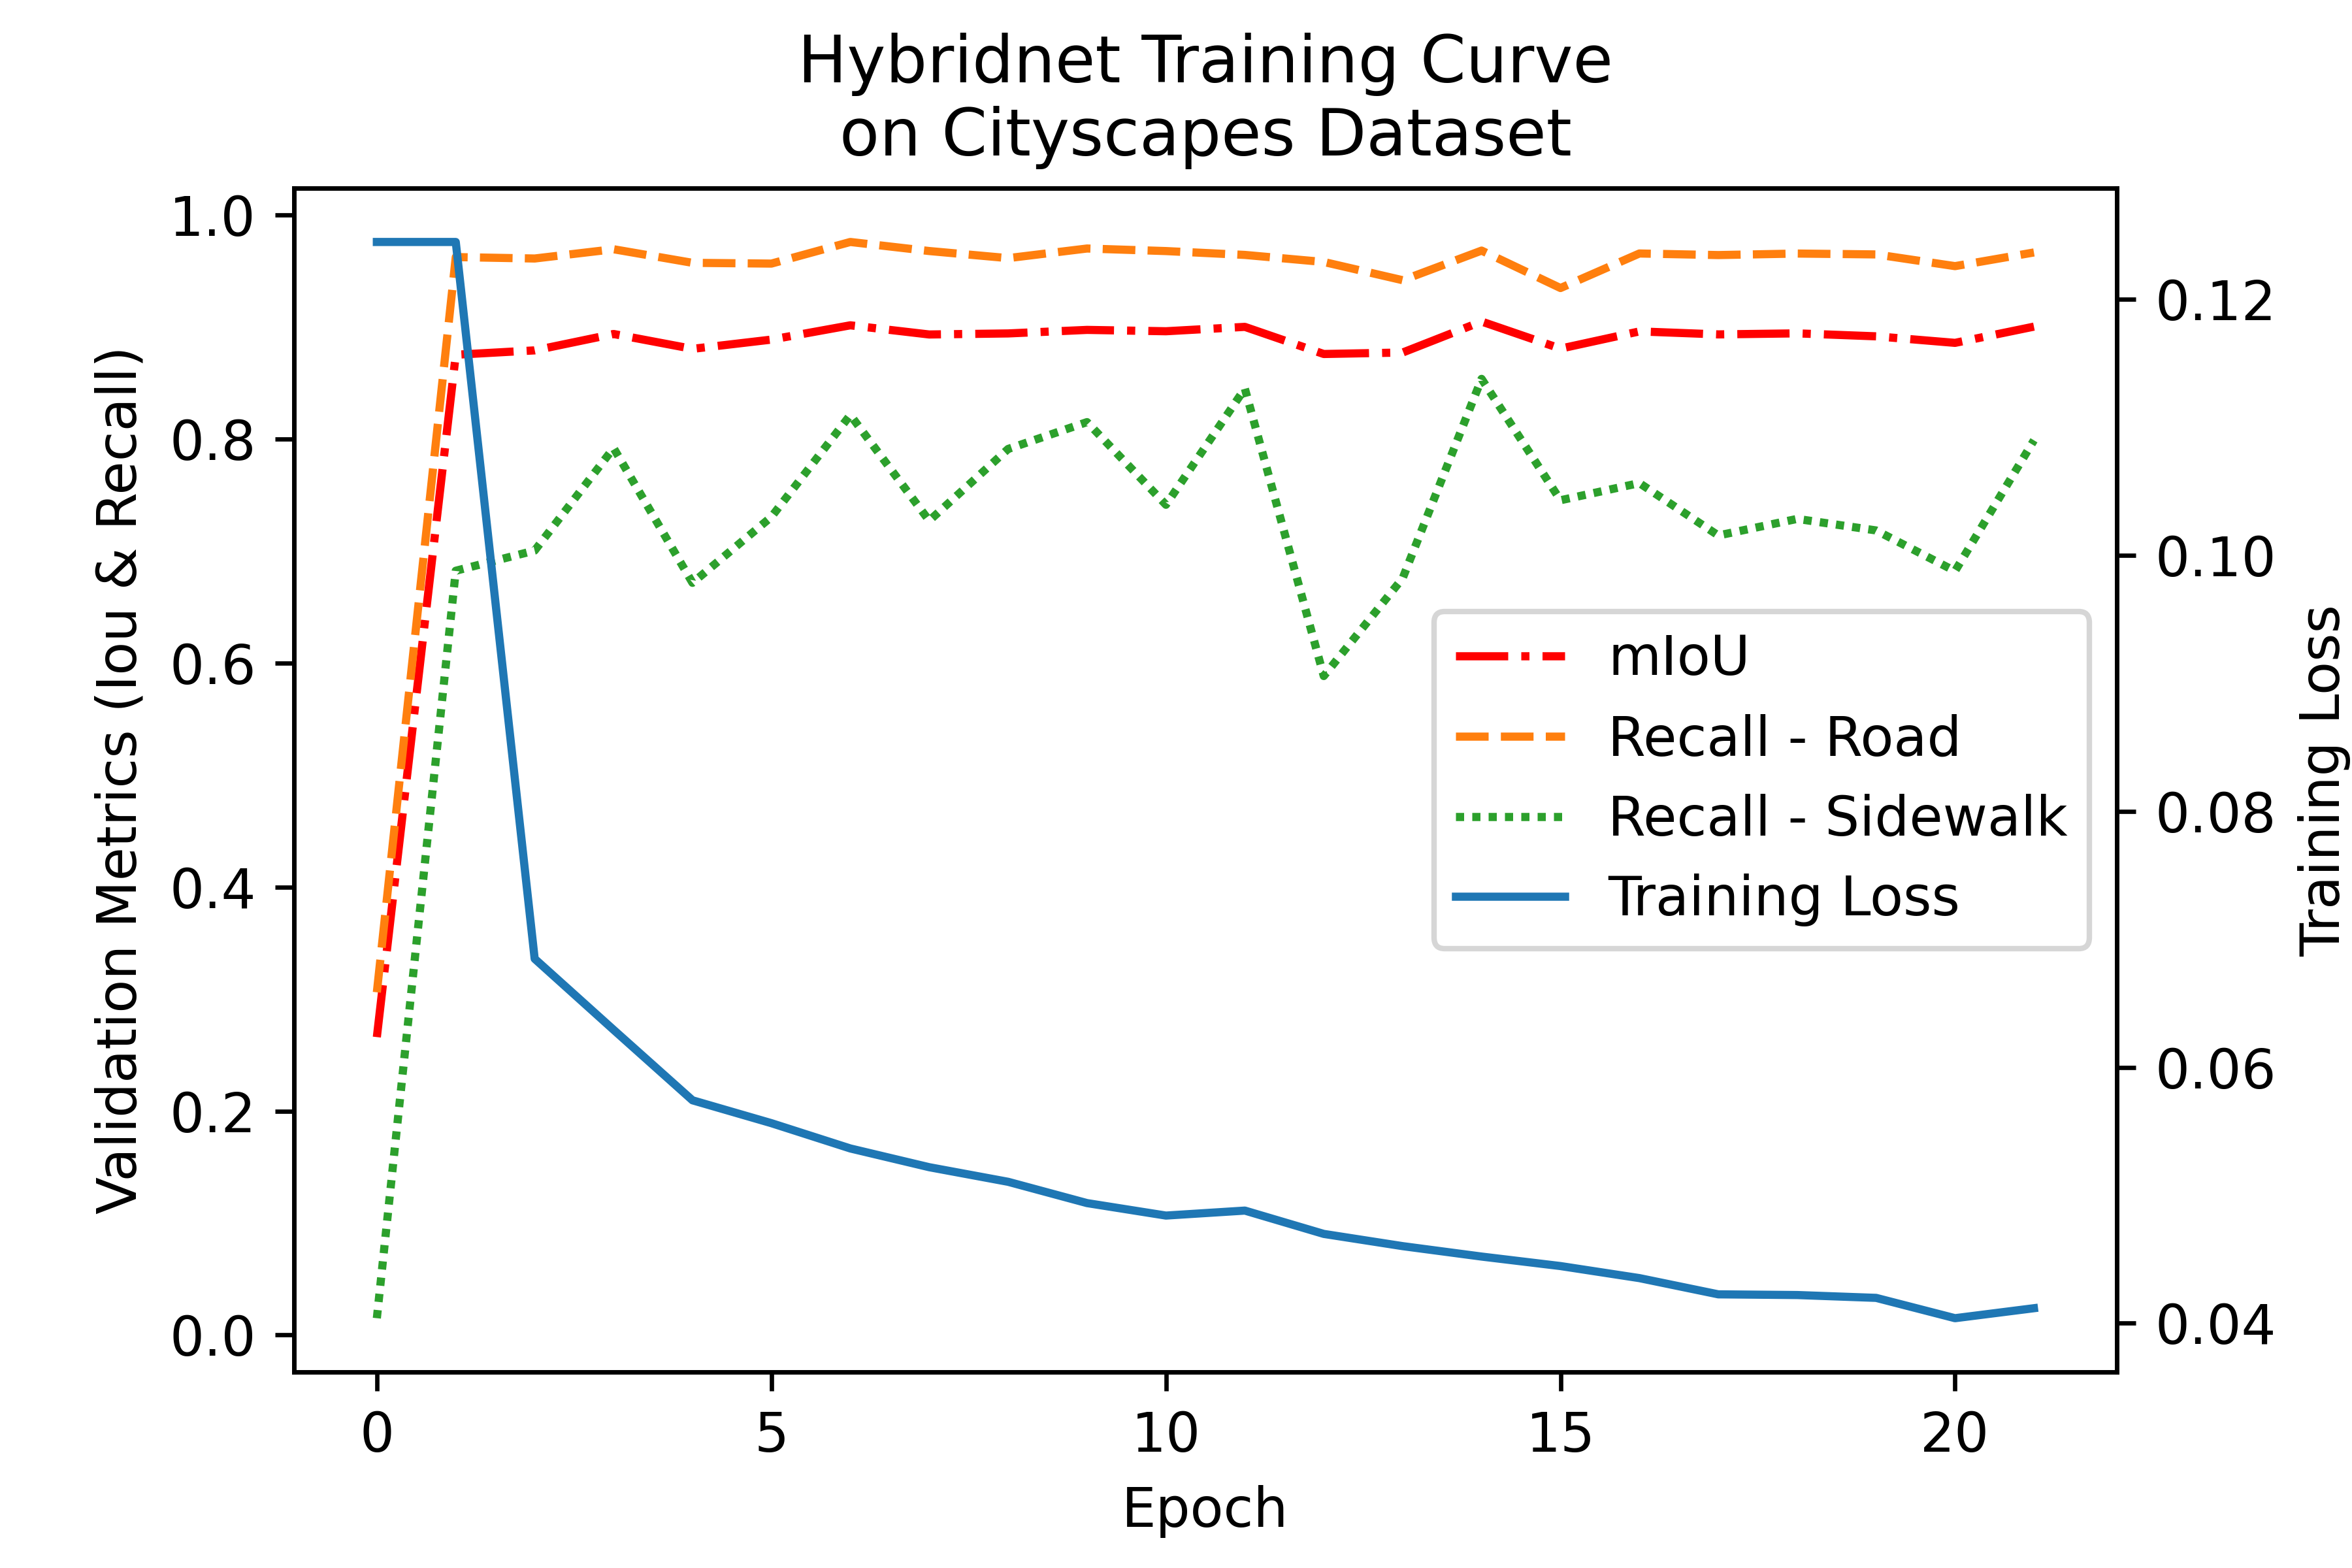
\includegraphics[width=0.6\linewidth]{images/hybridnet_training_curve.png}
    \caption{Hybridnets training curve}
    \label{fig:hybridnet_training_curve}
\end{figure}

\begin{figure}[b]
    % 16:6 width ratio
    % 0.64, 0.24
    \centering
    \begin{subfigure}{.4\textwidth}
        \centering
        \includegraphics[width=\linewidth]{images/hybridnets_untrained.PNG}
        \caption{Before retraining}
    \end{subfigure}
    \quad
    \begin{subfigure}{.4\textwidth}
        \centering
        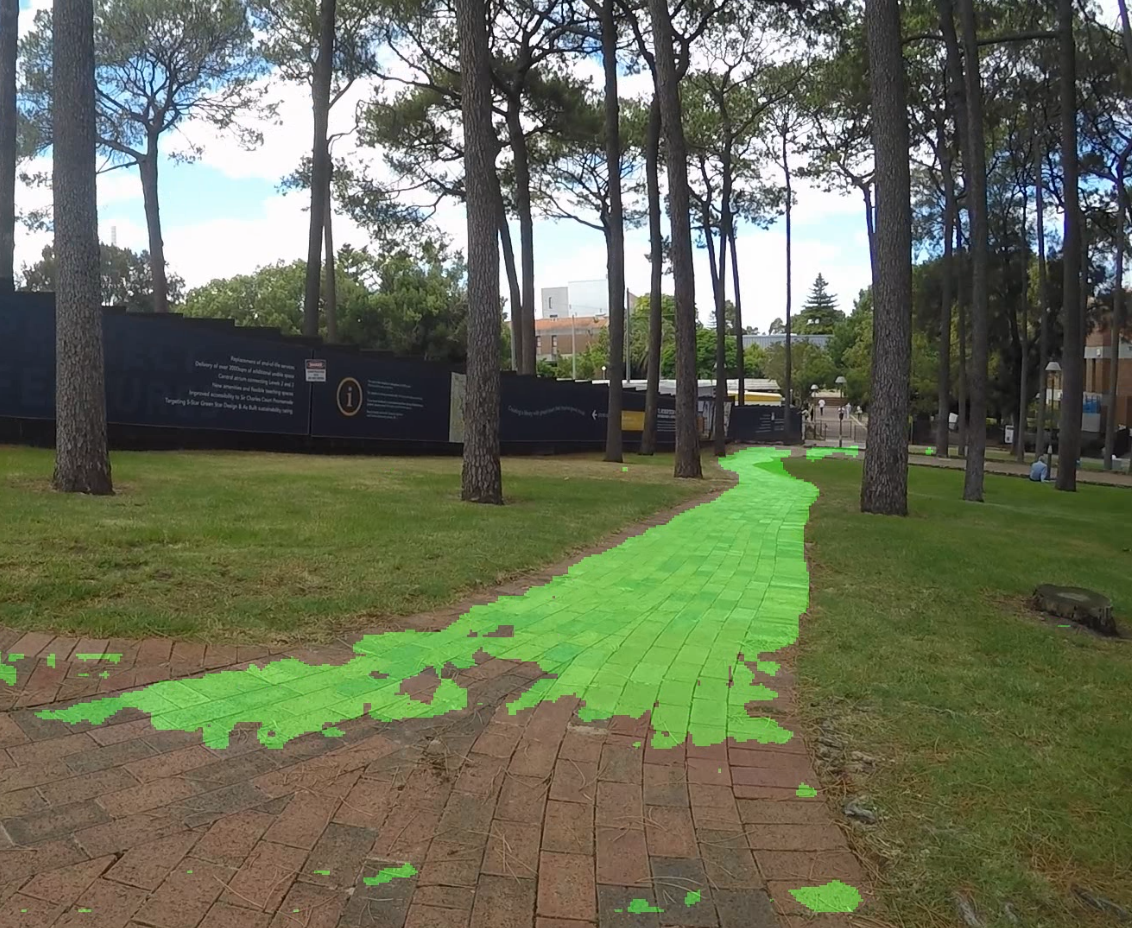
\includegraphics[width=\linewidth]{images/hybridnets_trained.PNG}
        \caption{After retraining}
    \end{subfigure}
    \caption{Hybridnets segmentation on the Curtin driving dataset (example 1)}
    \label{fig:compare_trained_hybridnets}
\end{figure}

\pagebreak
\subsection{Efficiacy of birds-eye view occupancy map transform}
Once the drivable area has been segmented, it is transformed into the XZ plane
as a birds-eye view occupancy map. This is done by processing the 3D point cloud
data from the ZED Mini camera.
Morphological processing is used to improve the density of this occupancy map.
An example of the segmented output alongside the occupancy map can be seen in \cref{fig:occupancy_map_seg},
with the drivable area highlighted in green.
Note that the occupancy map is 15 metres long and 10 metres wide. The location of the ZED Mini camera is depicted
with an `X'; the camera is mounted to the right-hand side of the wheelchair.

\begin{figure}[H]
    % 16:6 width ratio
    % 0.64, 0.24
    \centering
    \begin{subfigure}{.55\textwidth}
        \centering
        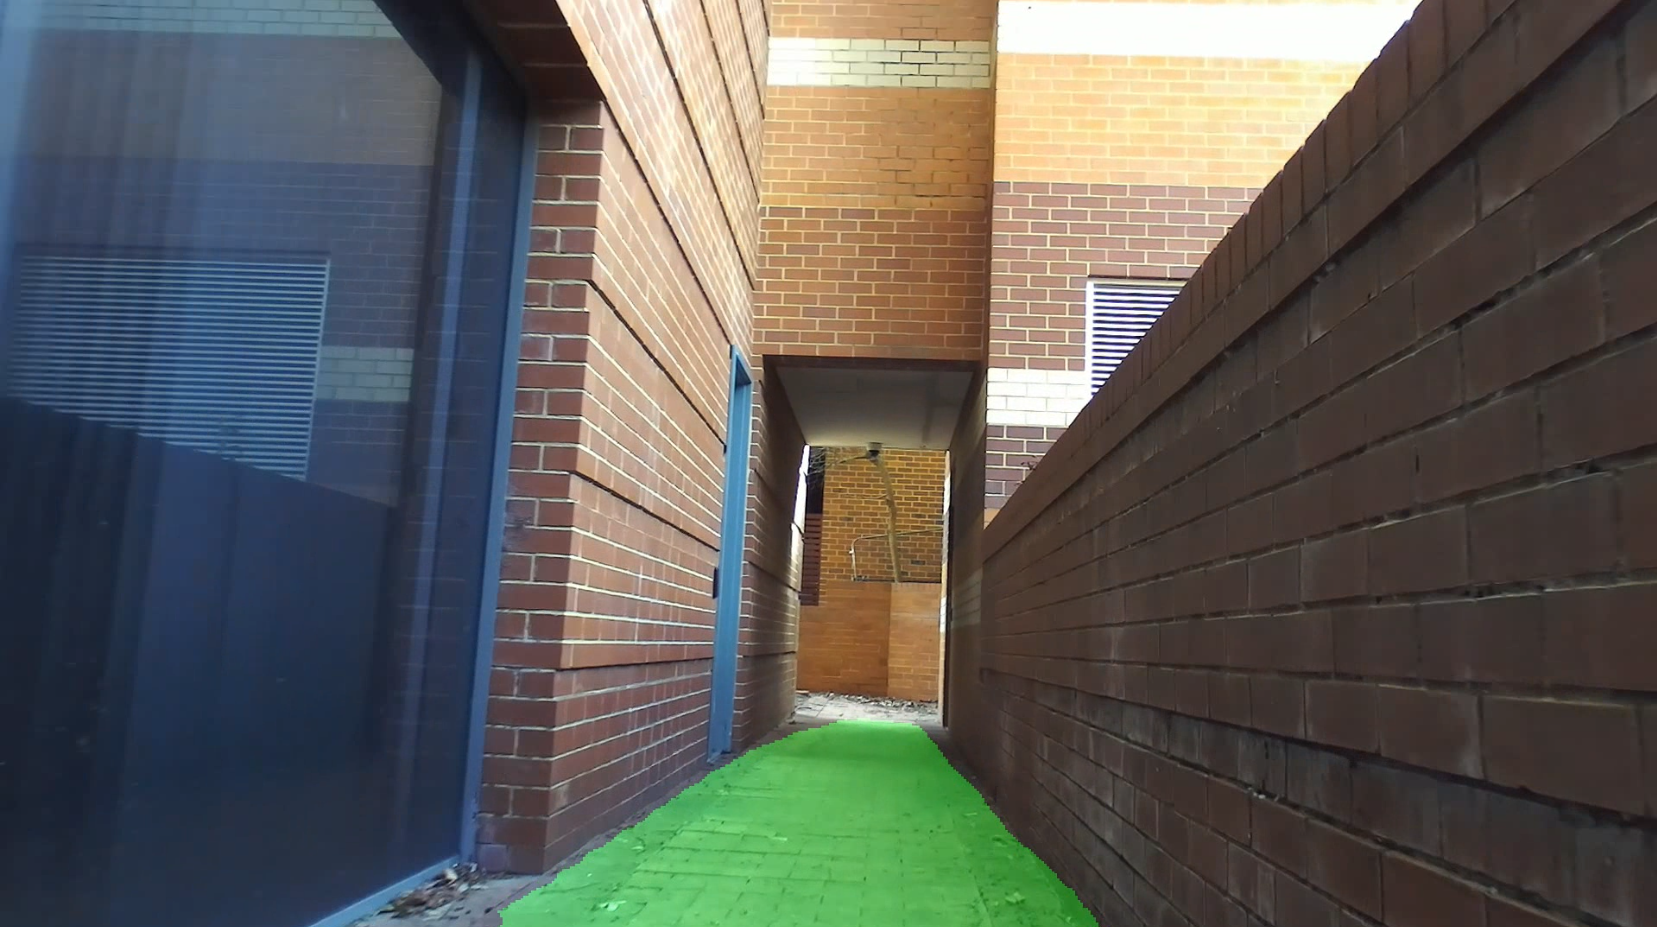
\includegraphics[width=\linewidth]{images/segmentation_1.PNG}
    \end{subfigure}
    \quad
    \begin{subfigure}{.2\textwidth}
        \centering
        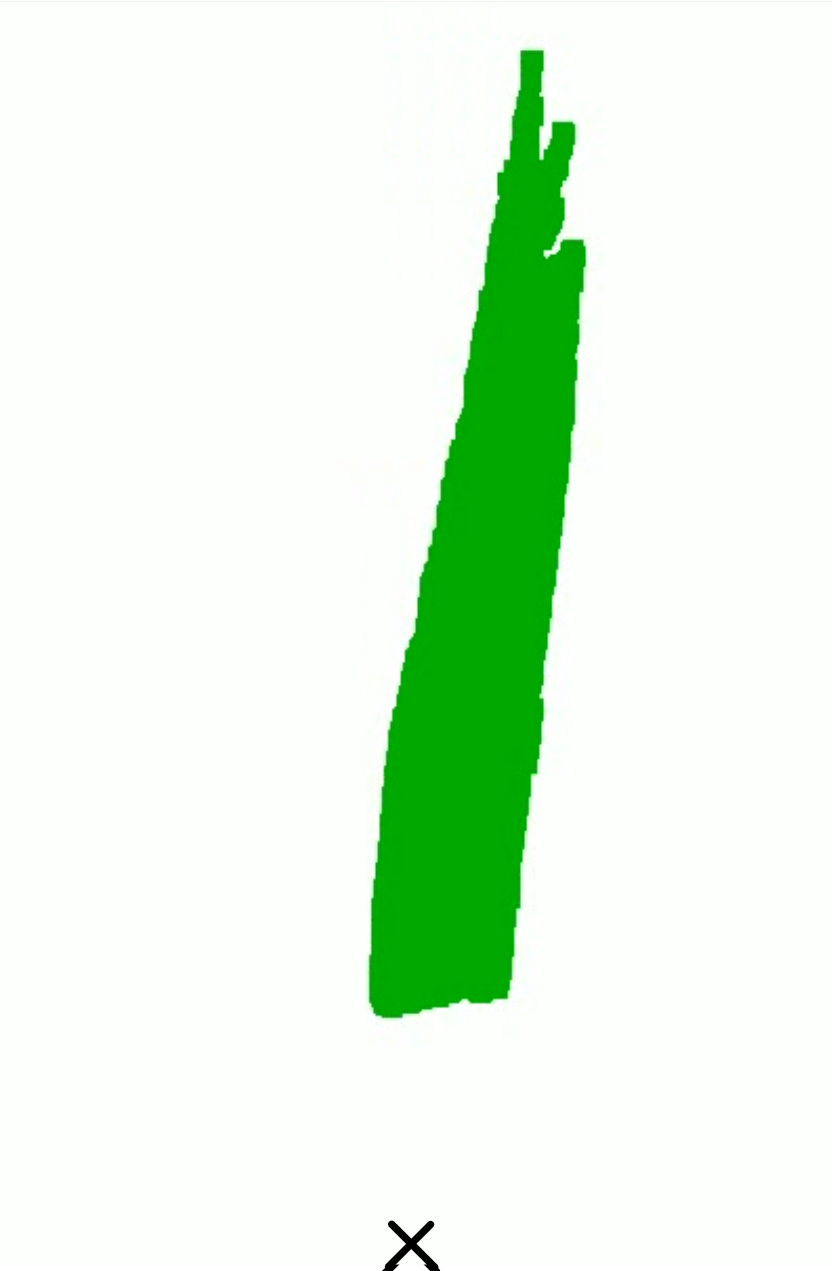
\includegraphics[width=\linewidth]{images/occupancy_map1.png}
    \end{subfigure}
    \smallskip
    \begin{subfigure}{.55\textwidth}
        \centering
        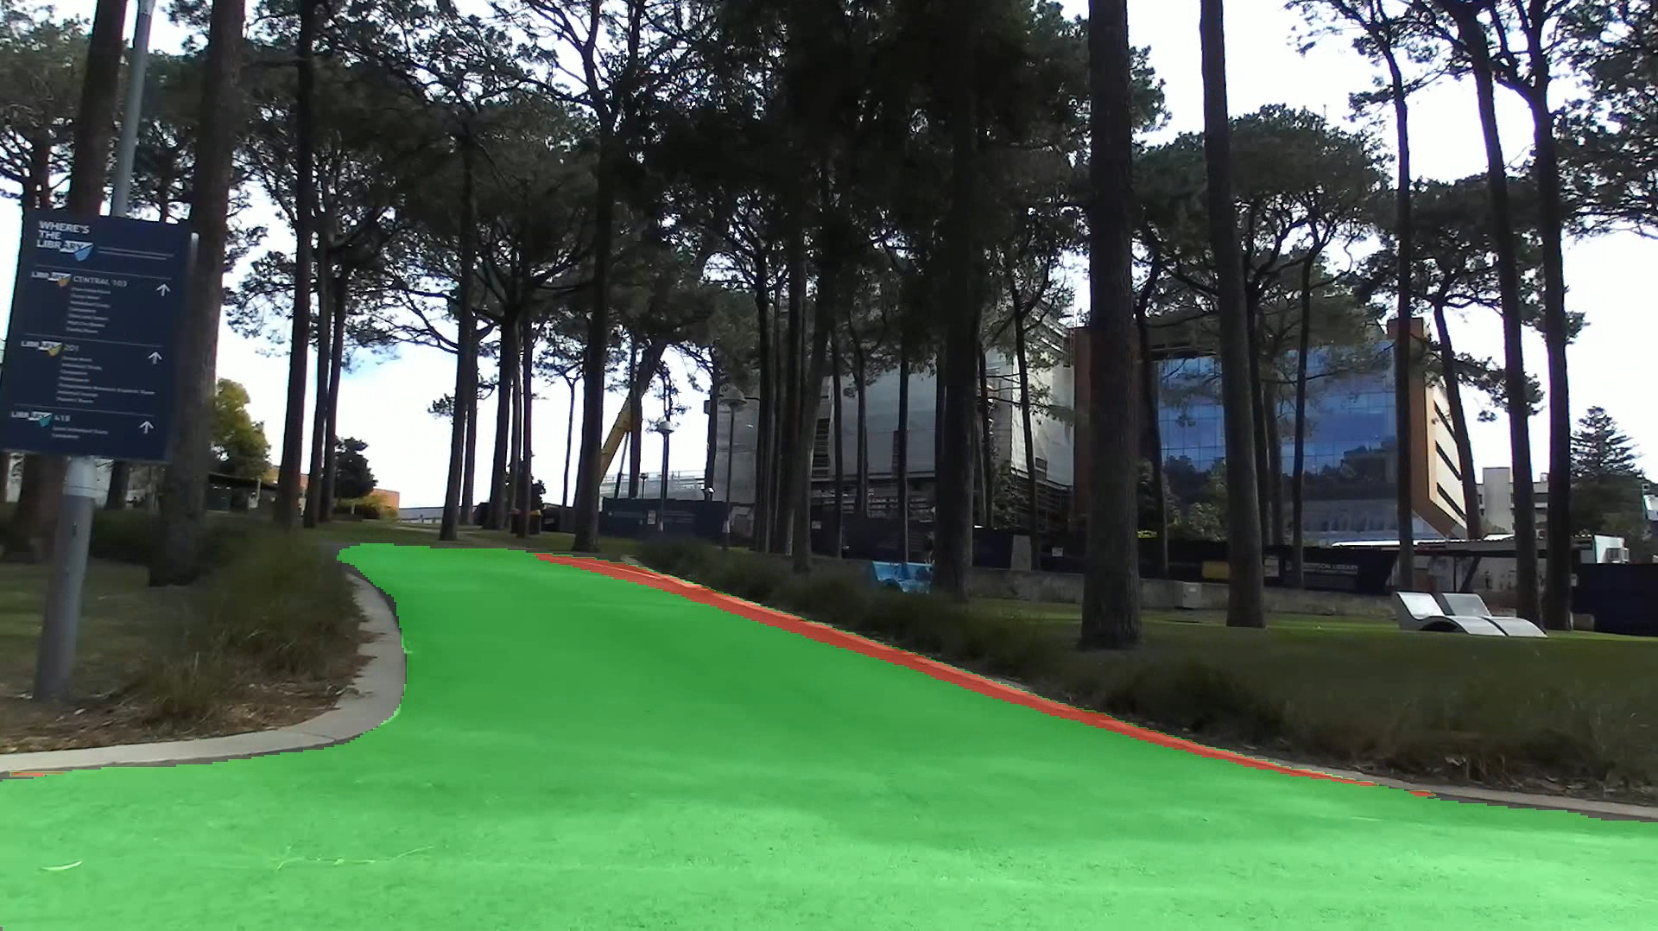
\includegraphics[width=\linewidth]{images/segmentation_2.PNG}
    \end{subfigure}
    \quad
    \begin{subfigure}{.2\textwidth}
        \centering
        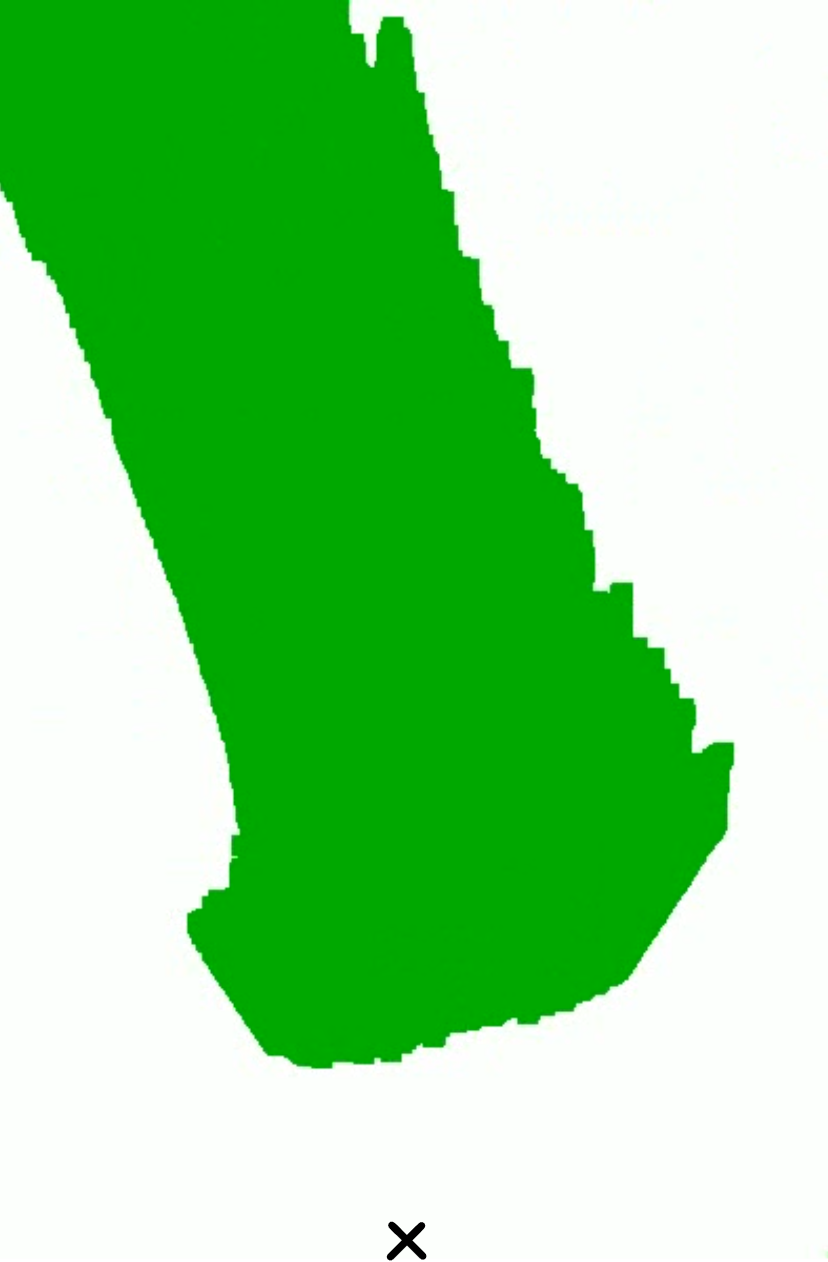
\includegraphics[width=\linewidth]{images/occupancy_map2.png}
    \end{subfigure}
    \smallskip
    \begin{subfigure}{.55\textwidth}
        \centering
        \includegraphics[width=\linewidth]{images/segmentation_3.PNG}
    \end{subfigure}
    \quad
    \begin{subfigure}{.2\textwidth}
        \centering
        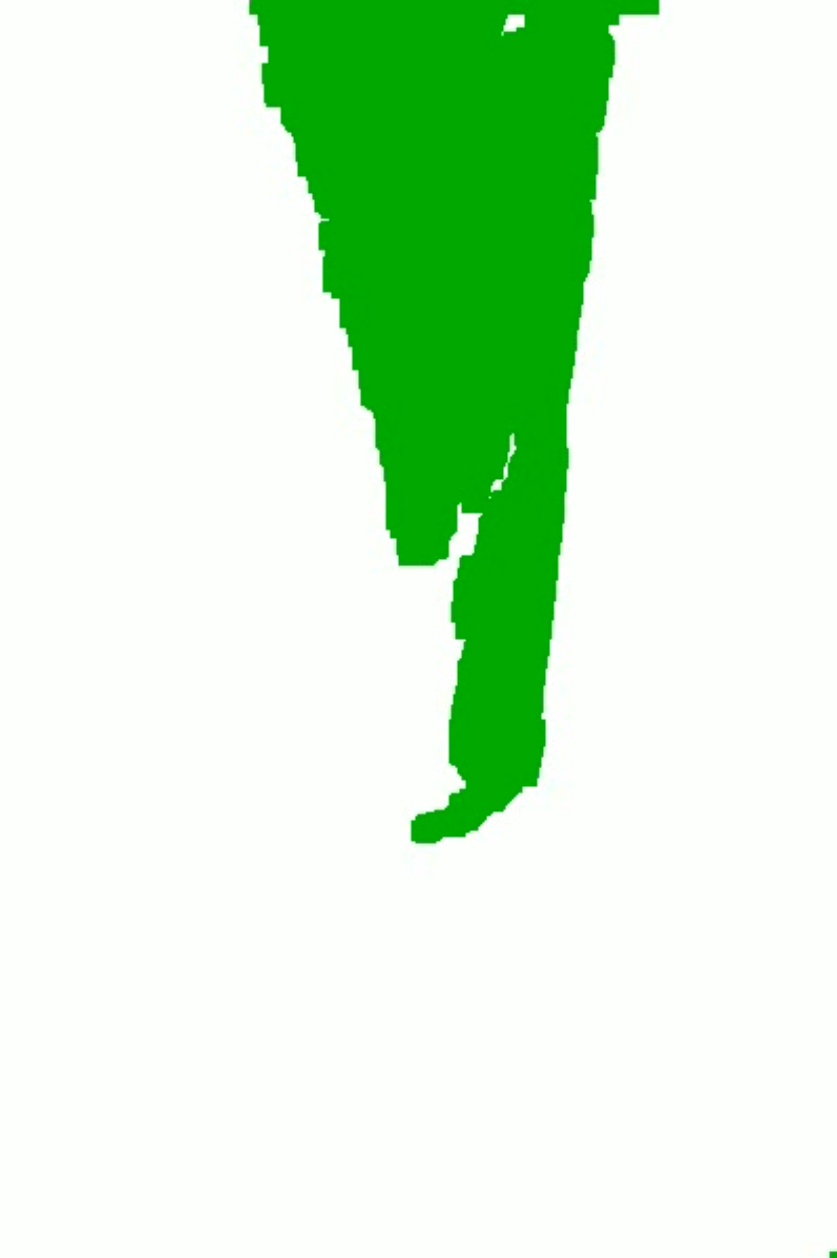
\includegraphics[width=\linewidth]{images/occupancy_map3.png}
    \end{subfigure}
    \caption{Segmented image output and corresponding occupancy map for three locations around Curtin university}
    \label{fig:occupancy_map_seg}
\end{figure}
\pagebreak

This segmented image to occupancy map transform works well in all observed cases, as long as the Hybridnets model identifies the
drivable area accurately. One improvement that could be made to this implementation is its speed.
The algorithm is bottlenecked by the occupancy map transform code, which takes between \SI{150}{\milli\second}
and \SI{500}{\milli\second} to execute, depending on the size of the drivable area.

Although this approach reliably maps drivable areas to an occupancy grid,
the area directly in front of the wheelchair (approx. \SI{2.6}{\metre}) and behind the wheelchair is unknown due to the FOV of the camera.
Several approaches to rectify this are explored in \cref{sec:future_work}.

A comparison of the occupancy map before and after morphological processing is shown in \cref{fig:morphological_processing}.
Although the occupancy map has a higher resolution before this transformation, the poor density of the map
could make it more difficult to process. The time taken to perform this morphological processing is negligible
when compared to other sections of this code.

\begin{figure}[b]
    % 16:6 width ratio
    % 0.64, 0.24
    \centering
    \begin{subfigure}{.4\textwidth}
        \centering
        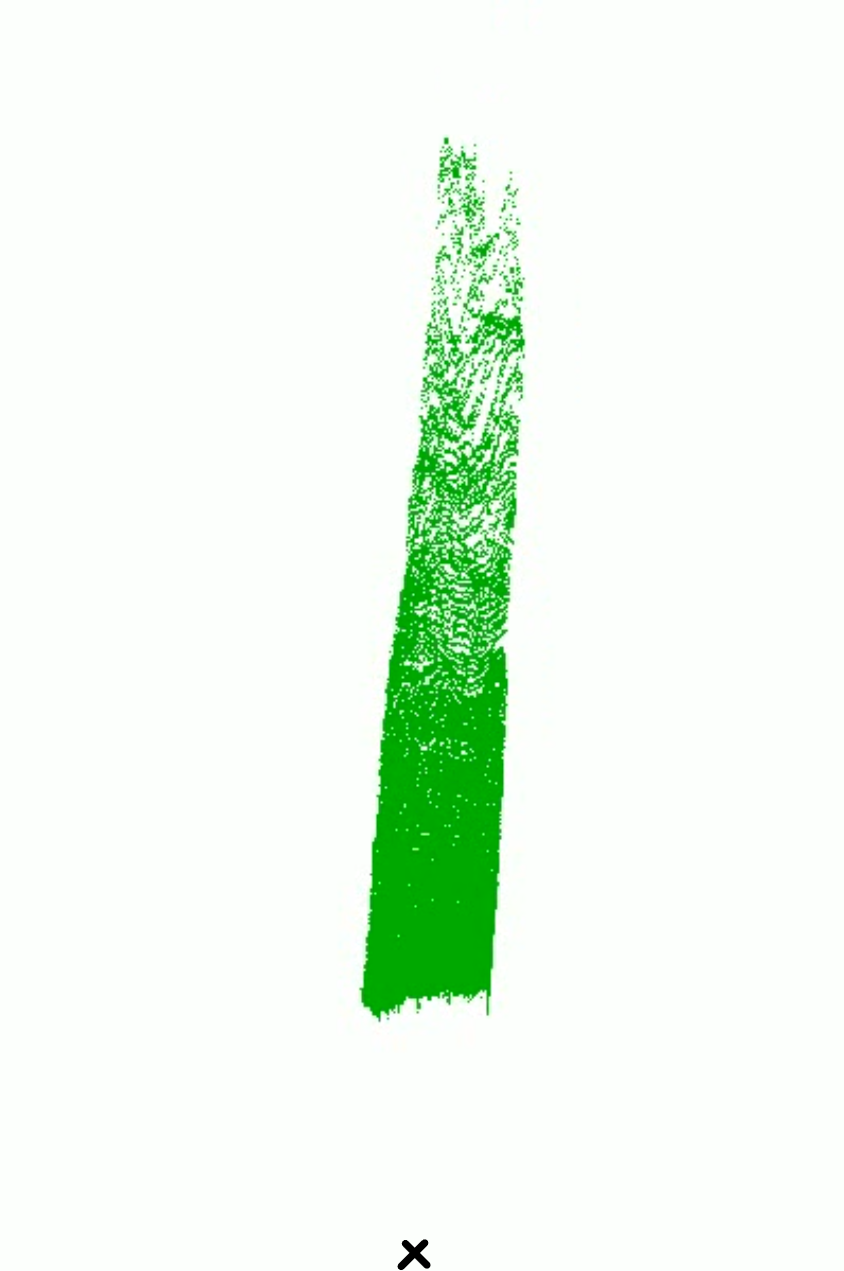
\includegraphics[width=\linewidth,frame]{images/occupancy_map1_nomorph.png}
        \caption{Before processing}
    \end{subfigure}
    \quad
    \begin{subfigure}{.4\textwidth}
        \centering
        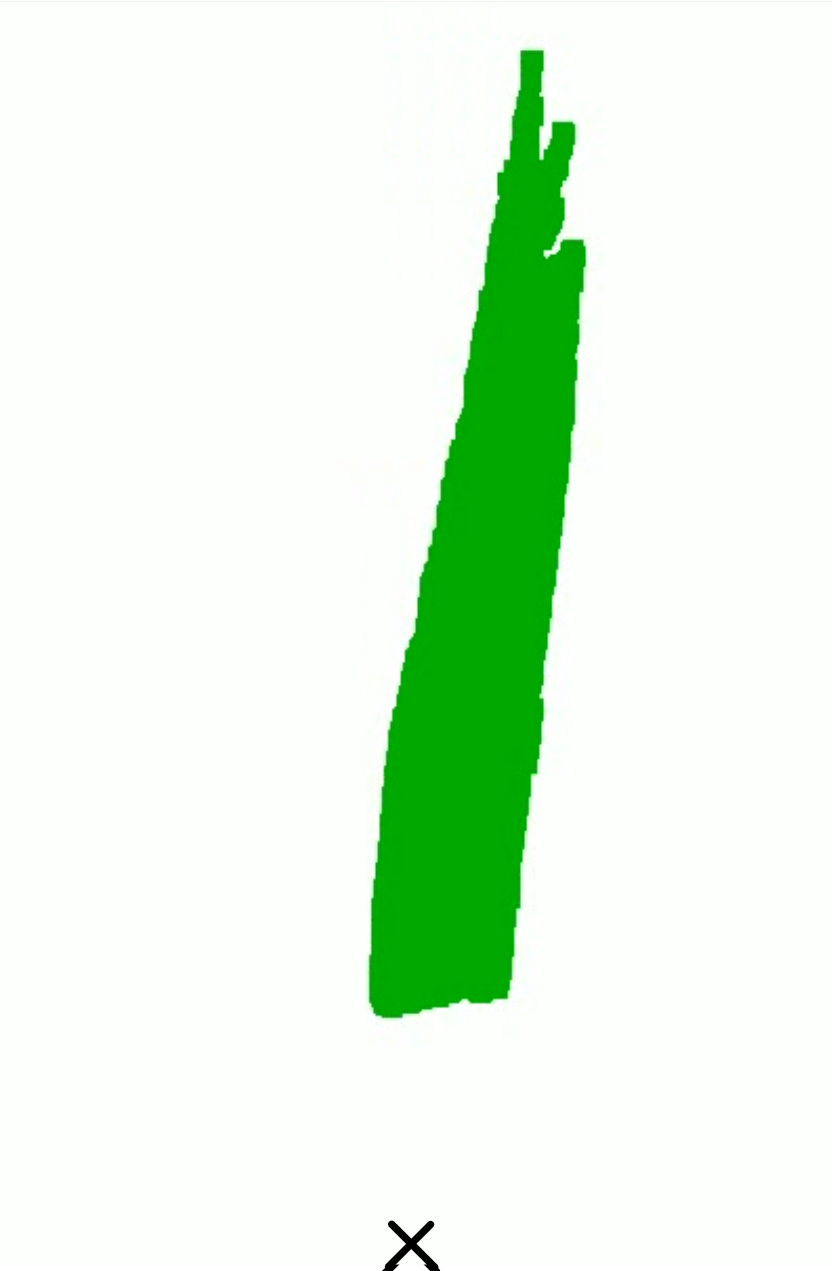
\includegraphics[width=\linewidth,frame]{images/occupancy_map1.png}
        \caption{After processing}
    \end{subfigure}
    \caption{Comparison of occupancy map before and after morphological processing}
    \label{fig:morphological_processing}
\end{figure}
\pagebreak
\subsection{Evaluation of 3D point cloud obstacle detection algorithms}
% sensor tilt, find_floor_plane
% compare performance vs ultra depth mode
Direct processing of the 3D point cloud data was tested to identify environmental obstacles and drivable areas.
One such approach involved using the inbuilt ZED SDK function \texttt{find\_floor\_plane},
which outputs a polygon of the floor plane.
This is shown in \cref{fig:find_floor_plane} and compared alongside the segmentation occupancy map.
This approach is very poor at identifying the floor plane accurately and has large frame-to-frame
variation in its output. The only redeeming factor of this approach is its speed;
as the function is GPU accelerated, this calculation takes approximately \SI{60}{\milli\second}.

\begin{figure}[b]
    % 16:6 width ratio
    % 0.64, 0.24
    \centering
    \begin{subfigure}{.5\textwidth}
        \centering
        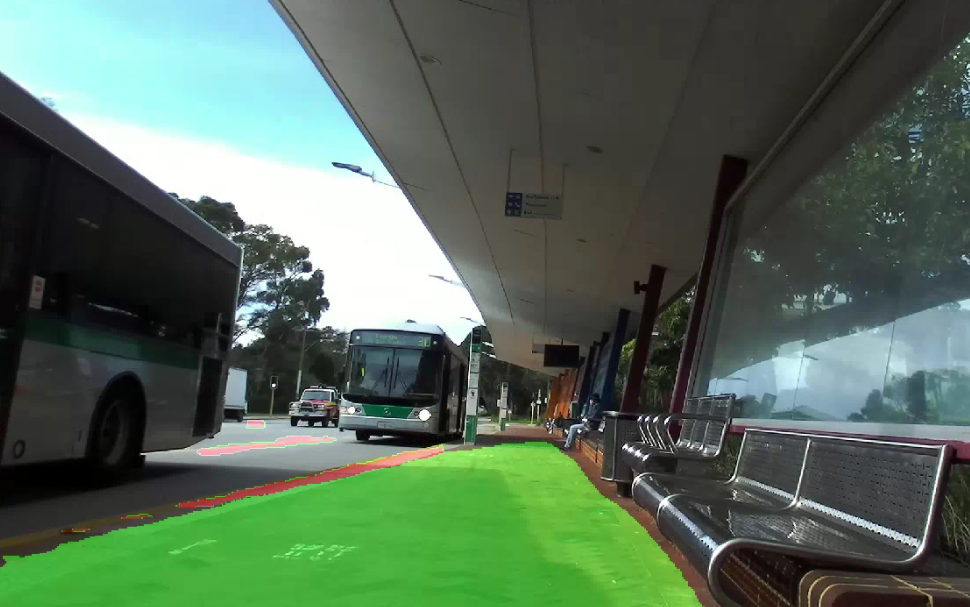
\includegraphics[width=\linewidth]{images/find_floor_plane_video.PNG}
        \caption{Video footage}
    \end{subfigure}
    \quad
    \begin{subfigure}{.2\textwidth}
        \centering
        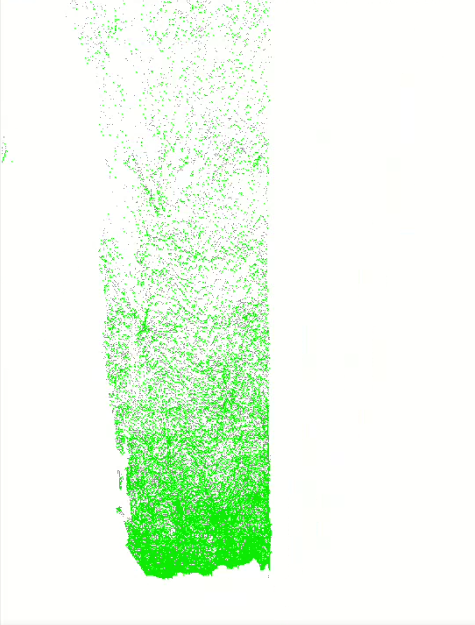
\includegraphics[width=\linewidth,frame]{images/find_floor_plane_seg.PNG}
        \caption{Segmentation occupancy map}
    \end{subfigure}
    \quad
    \begin{subfigure}{.2\textwidth}
        \centering
        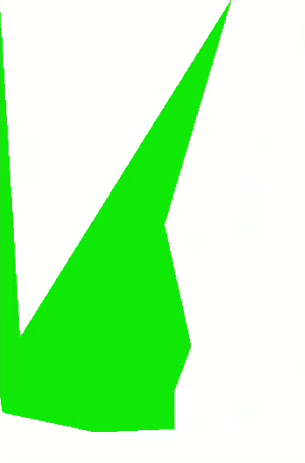
\includegraphics[width=\linewidth,frame]{images/find_floor_plane.PNG}
        \caption{Output from \texttt{find\_floor\_plane}}
    \end{subfigure}
    \caption{ZED SDK \texttt{find\_floor\_plane} function compared with segmentation occupancy map}
    \label{fig:find_floor_plane}
\end{figure}

Another approach that was tested was a custom algorithm to process the point cloud data,
detailed in \cref{sec:point_cloud_obstacle_detection}. The results of this algorithm
are shown in three scenarios: one indoor (\cref{fig:pcloud_indoor}) and two outdoor (\cref{fig:pcloud_outdoor_bad} and \cref{fig:pcloud_outdoor_good}).
Note that the drivable area is labelled in green and the environmental obstacles are labelled in red.

This algorithm works well in indoor settings (\cref{fig:pcloud_indoor}) at identifying the drivable area
as well as the position of walls and other static objects. Accurate occupancy maps are also generated for
outdoor settings with well-defined boundaries, such as a wheelchair ramp with handrails (\cref{fig:pcloud_outdoor_good}).
However, this algorithm can struggle with open outdoor settings as seen in \cref{fig:pcloud_outdoor_bad}.
Due to the uniformity of the pedestrian path in this image, the ZED Mini is unable to
reliably generate a depth map and 3D point cloud for the path. This leads to the algorithm
mistakenly identifying grassy and uneven terrain as drivable, but not identifying the
path as drivable.

This algorithm is slower than the segmentation approach, with a mean latency of \SI{550}{\milli\second}.
Due to this limitation, it is more suited for identifying non-moving objects such as walls
as opposed to identifying moving objects such as people and vehicles.

% squeeze in!
\begin{figure}[p]
    % 16:6 width ratio
    % 0.64, 0.24
    % 0.48, 0.18
    \centering
    \begin{subfigure}{.6\textwidth}
        \centering
        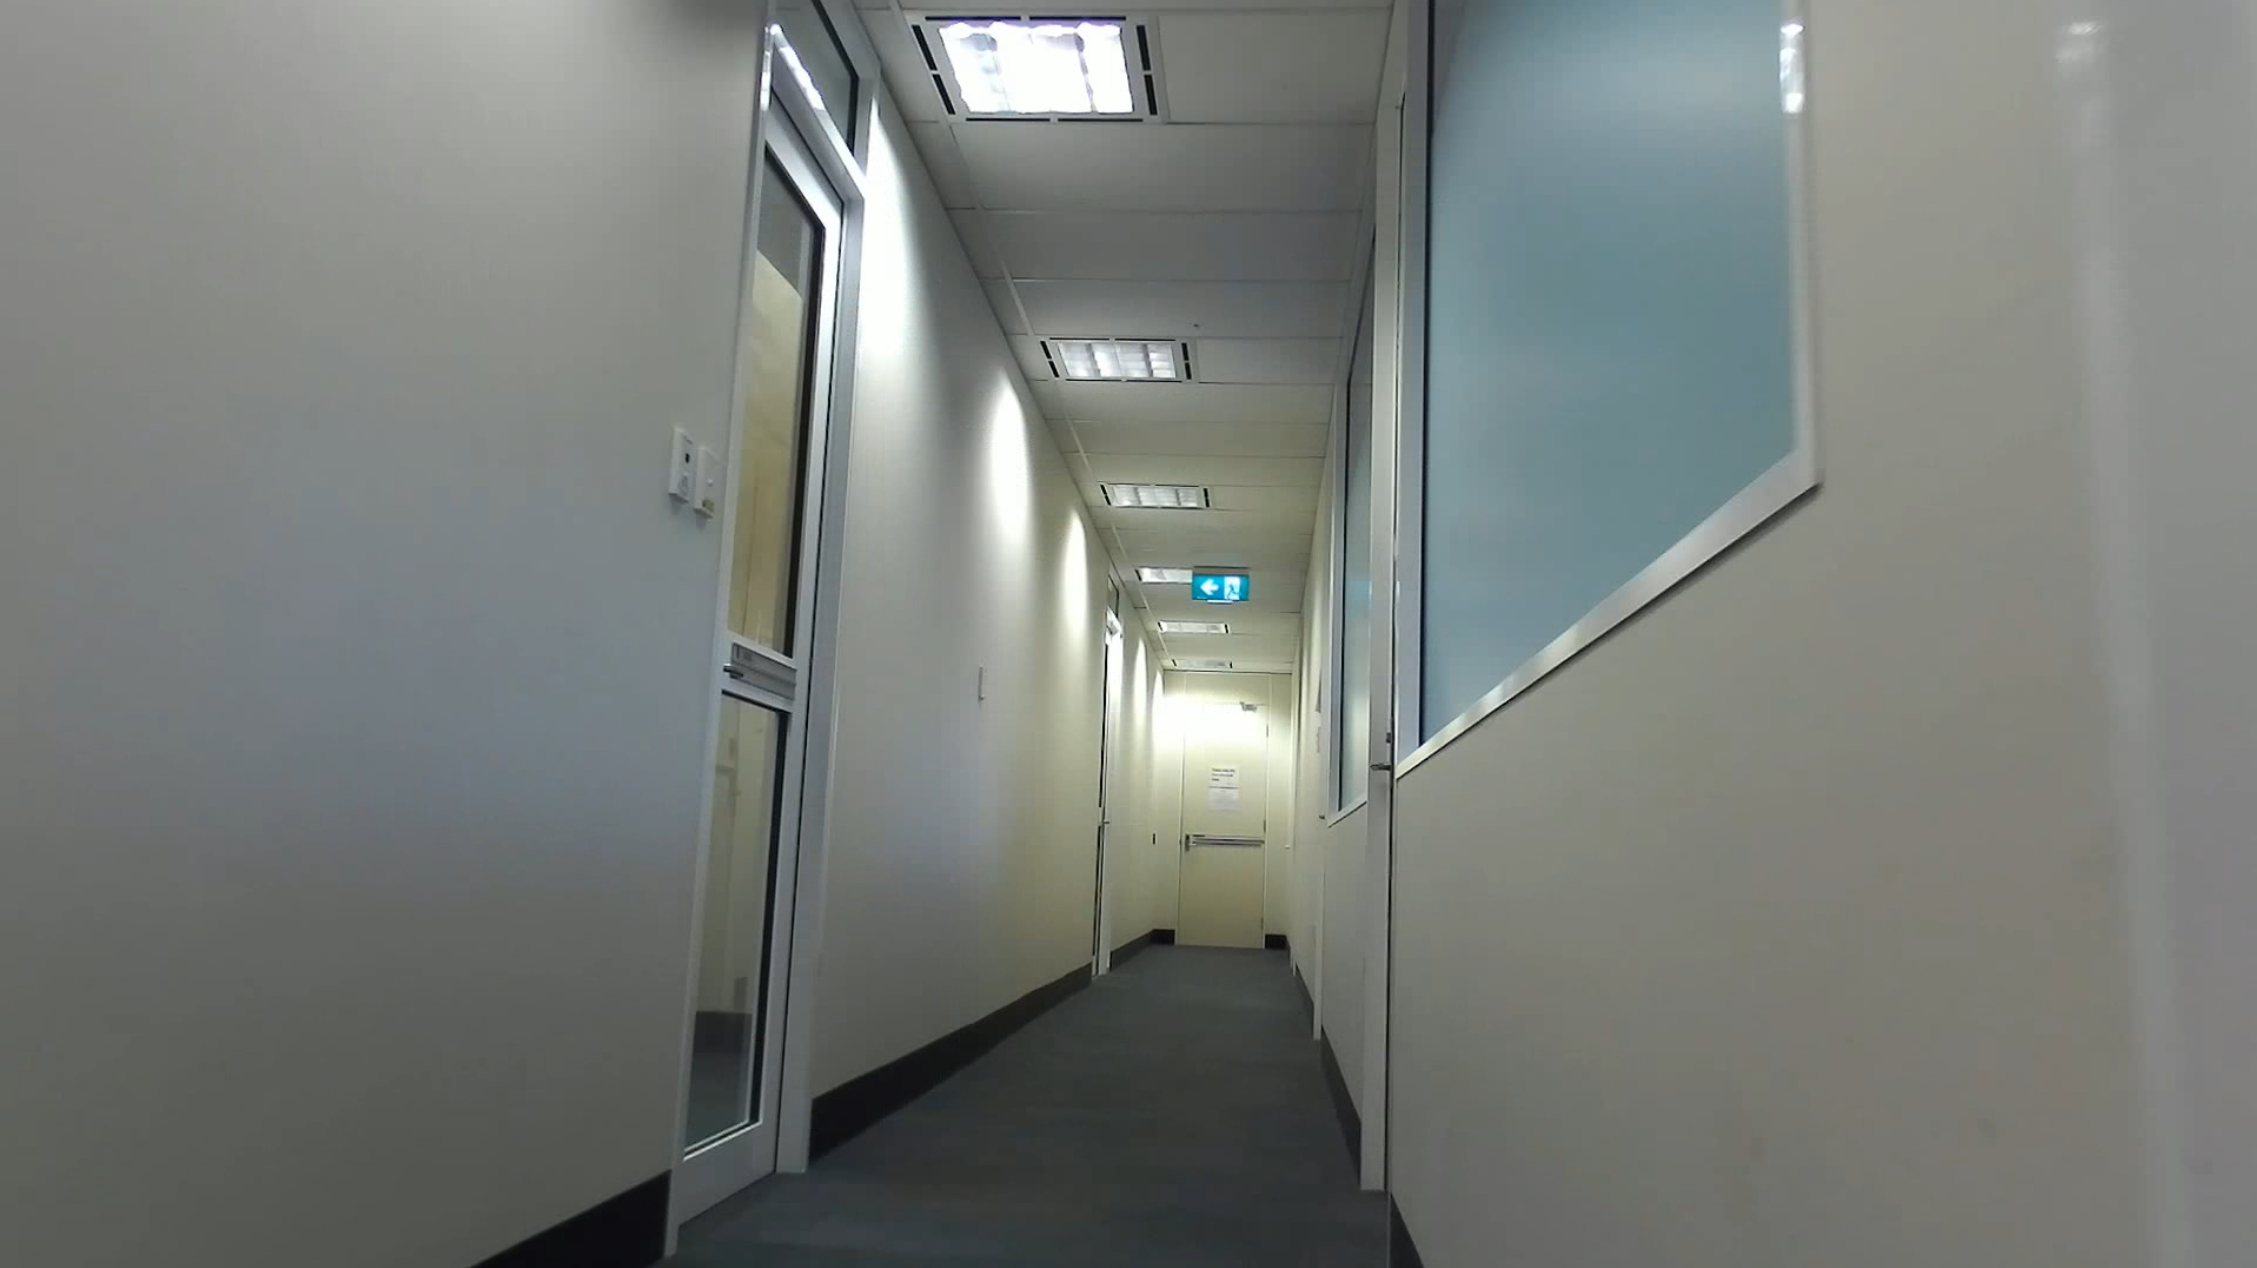
\includegraphics[width=\linewidth]{images/pcloud_indoor_video.PNG}
        \caption{Video footage}
    \end{subfigure}
    \quad
    \begin{subfigure}{.3\textwidth}
        \centering
        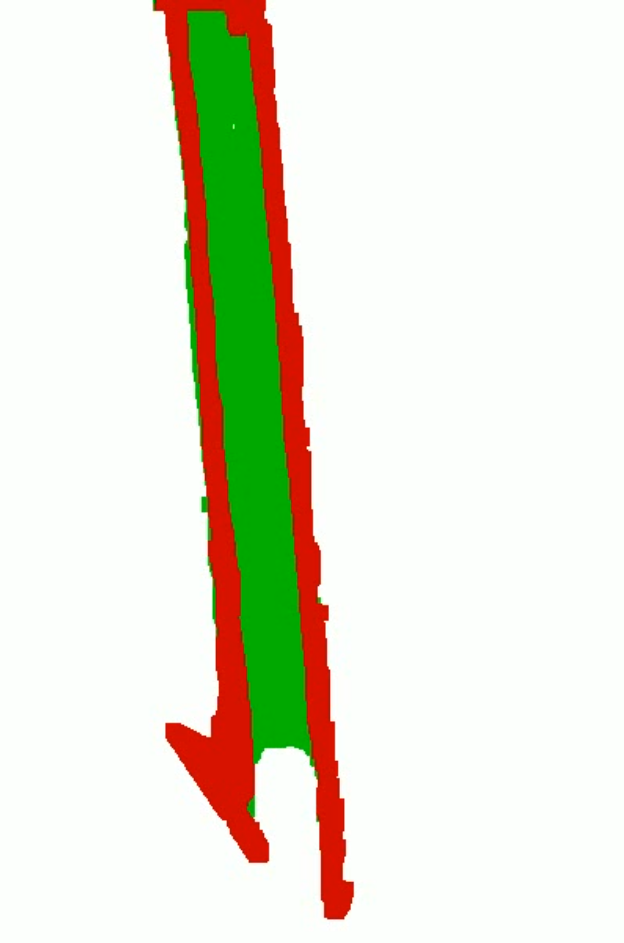
\includegraphics[width=\linewidth,frame]{images/pcloud_indoor.PNG}
        \caption{Occupancy map}
    \end{subfigure}
    \caption{Point cloud processing result (Indoor)}
    \label{fig:pcloud_indoor}
\end{figure}

\begin{figure}[p]
    % 16:6 width ratio
    % 0.64, 0.24
    \centering
    \begin{subfigure}{.6\textwidth}
        \centering
        \includegraphics[width=\linewidth]{images/pcloud_outdoor_bad_video.PNG}
        \caption{Video footage}
    \end{subfigure}
    \quad
    \begin{subfigure}{.3\textwidth}
        \centering
        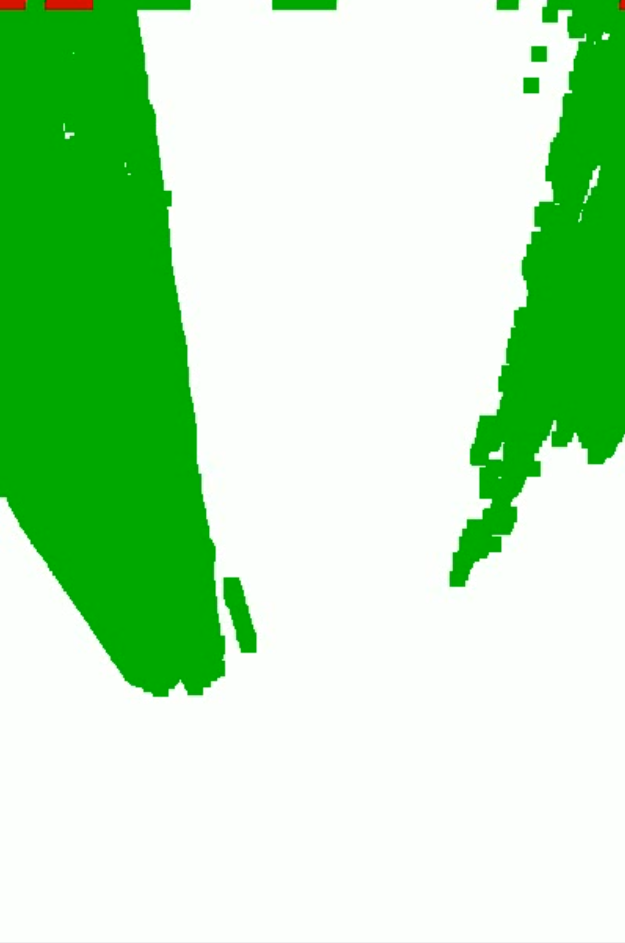
\includegraphics[width=\linewidth,frame]{images/pcloud_outdoor_bad.PNG}
        \caption{Occupancy map}
    \end{subfigure}
    \caption{Point cloud processing result (Outdoor, uniform path)}
    \label{fig:pcloud_outdoor_bad}
\end{figure}\clearpage

\begin{figure}[p]
    % 16:6 width ratio
    % 0.64, 0.24
    \centering
    \begin{subfigure}{.6\textwidth}
        \centering
        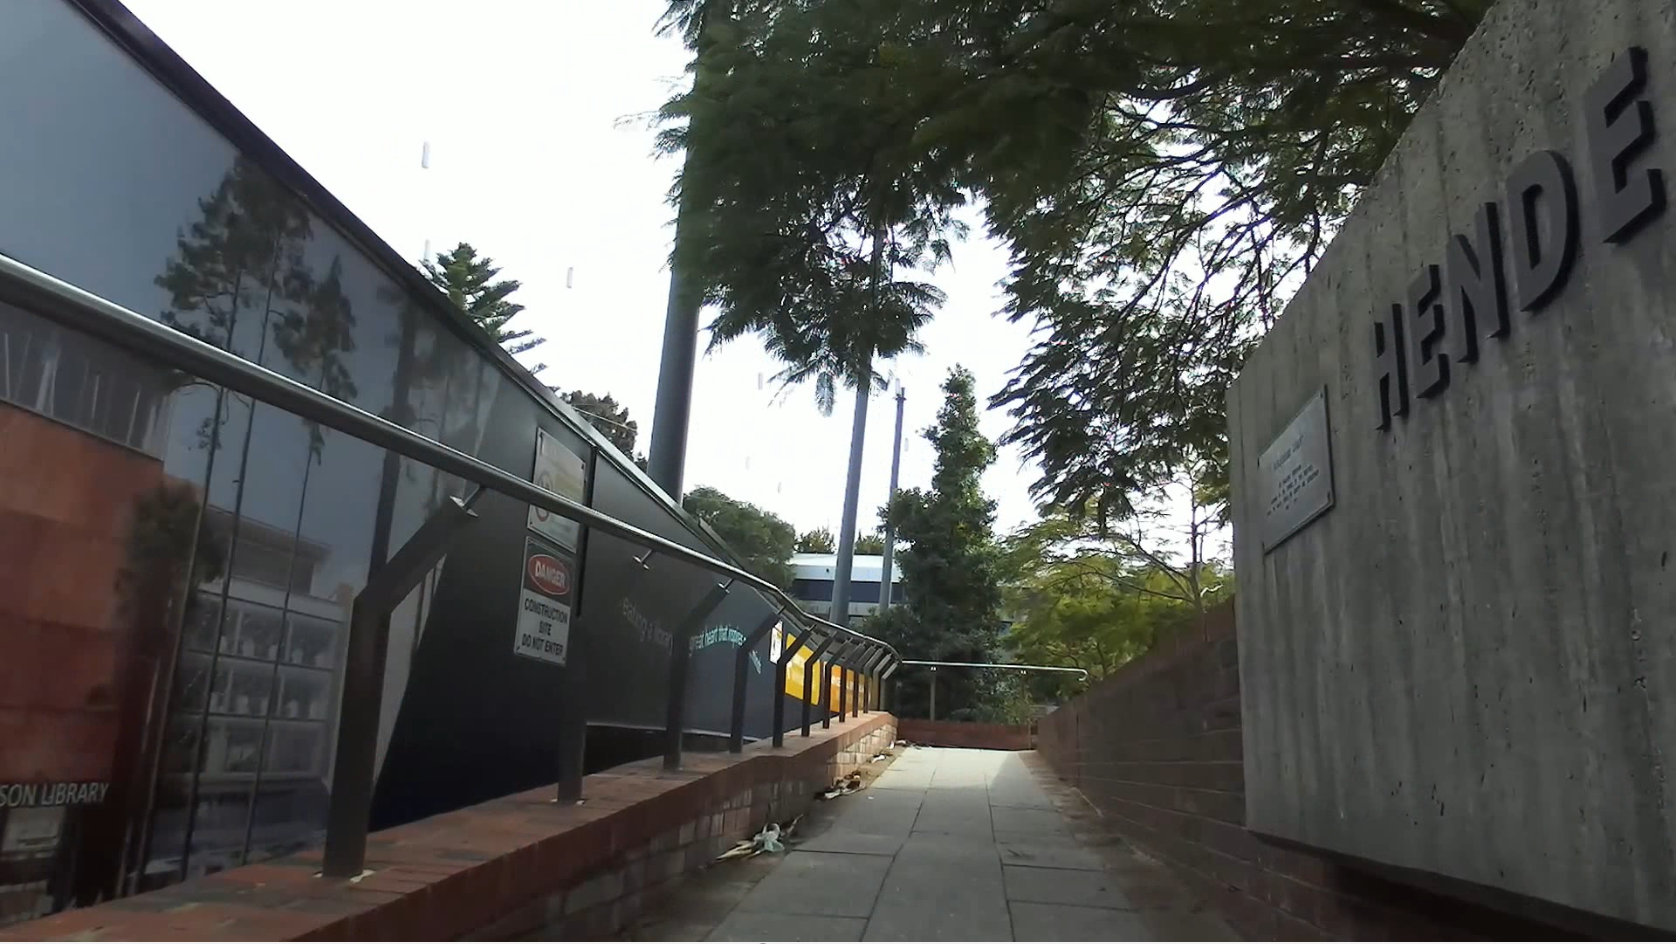
\includegraphics[width=\linewidth]{images/pcloud_outdoor_good_video.PNG}
        \caption{Video footage}
    \end{subfigure}
    \quad
    \begin{subfigure}{.3\textwidth}
        \centering
        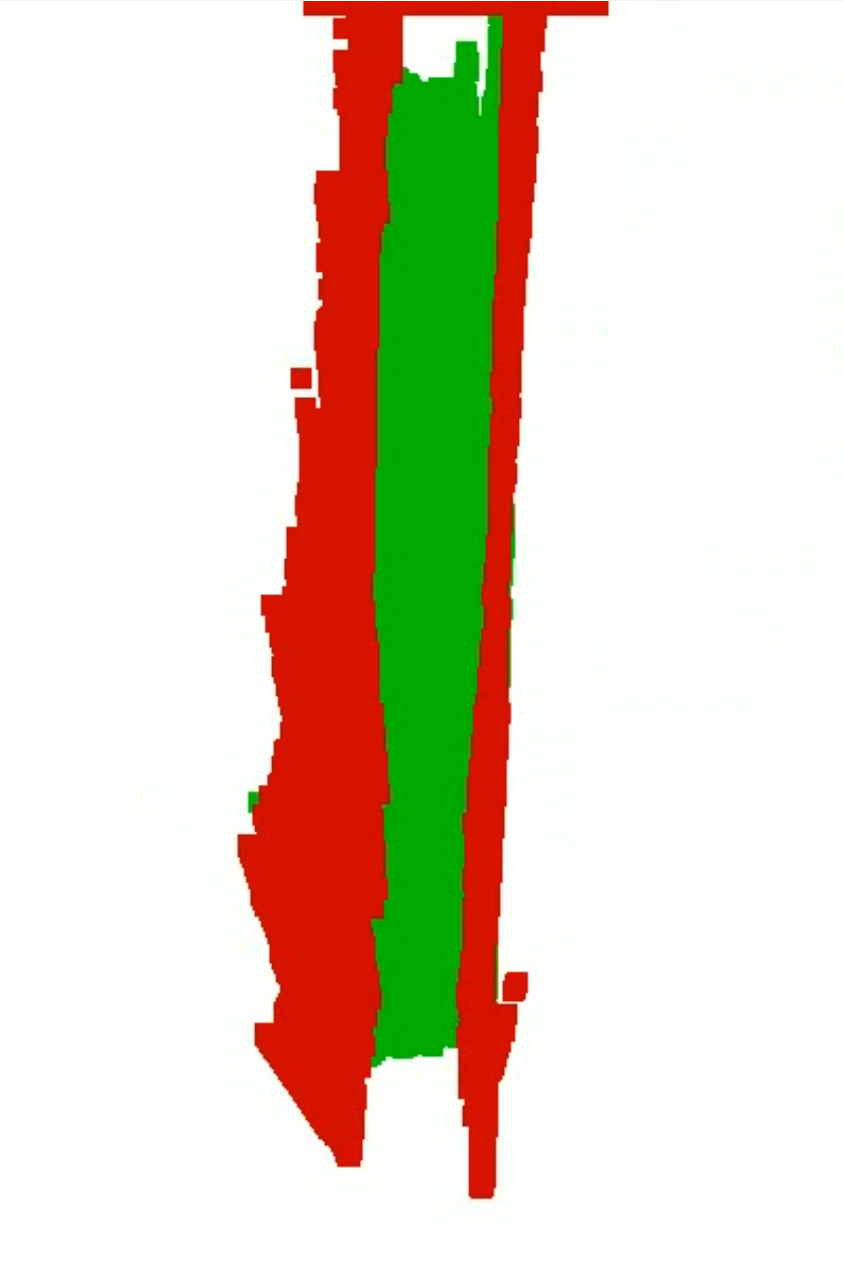
\includegraphics[width=\linewidth,frame]{images/pcloud_outdoor_good.PNG}
        \caption{Occupancy map}
    \end{subfigure}
    \caption{Point cloud processing result (Outdoor, wheelchair ramp)}
    \label{fig:pcloud_outdoor_good}
\end{figure}

\begin{figure}[p]
    % 16:6 width ratio
    % 0.64, 0.24
    \centering
    \begin{subfigure}{.55\textwidth}
        \centering
        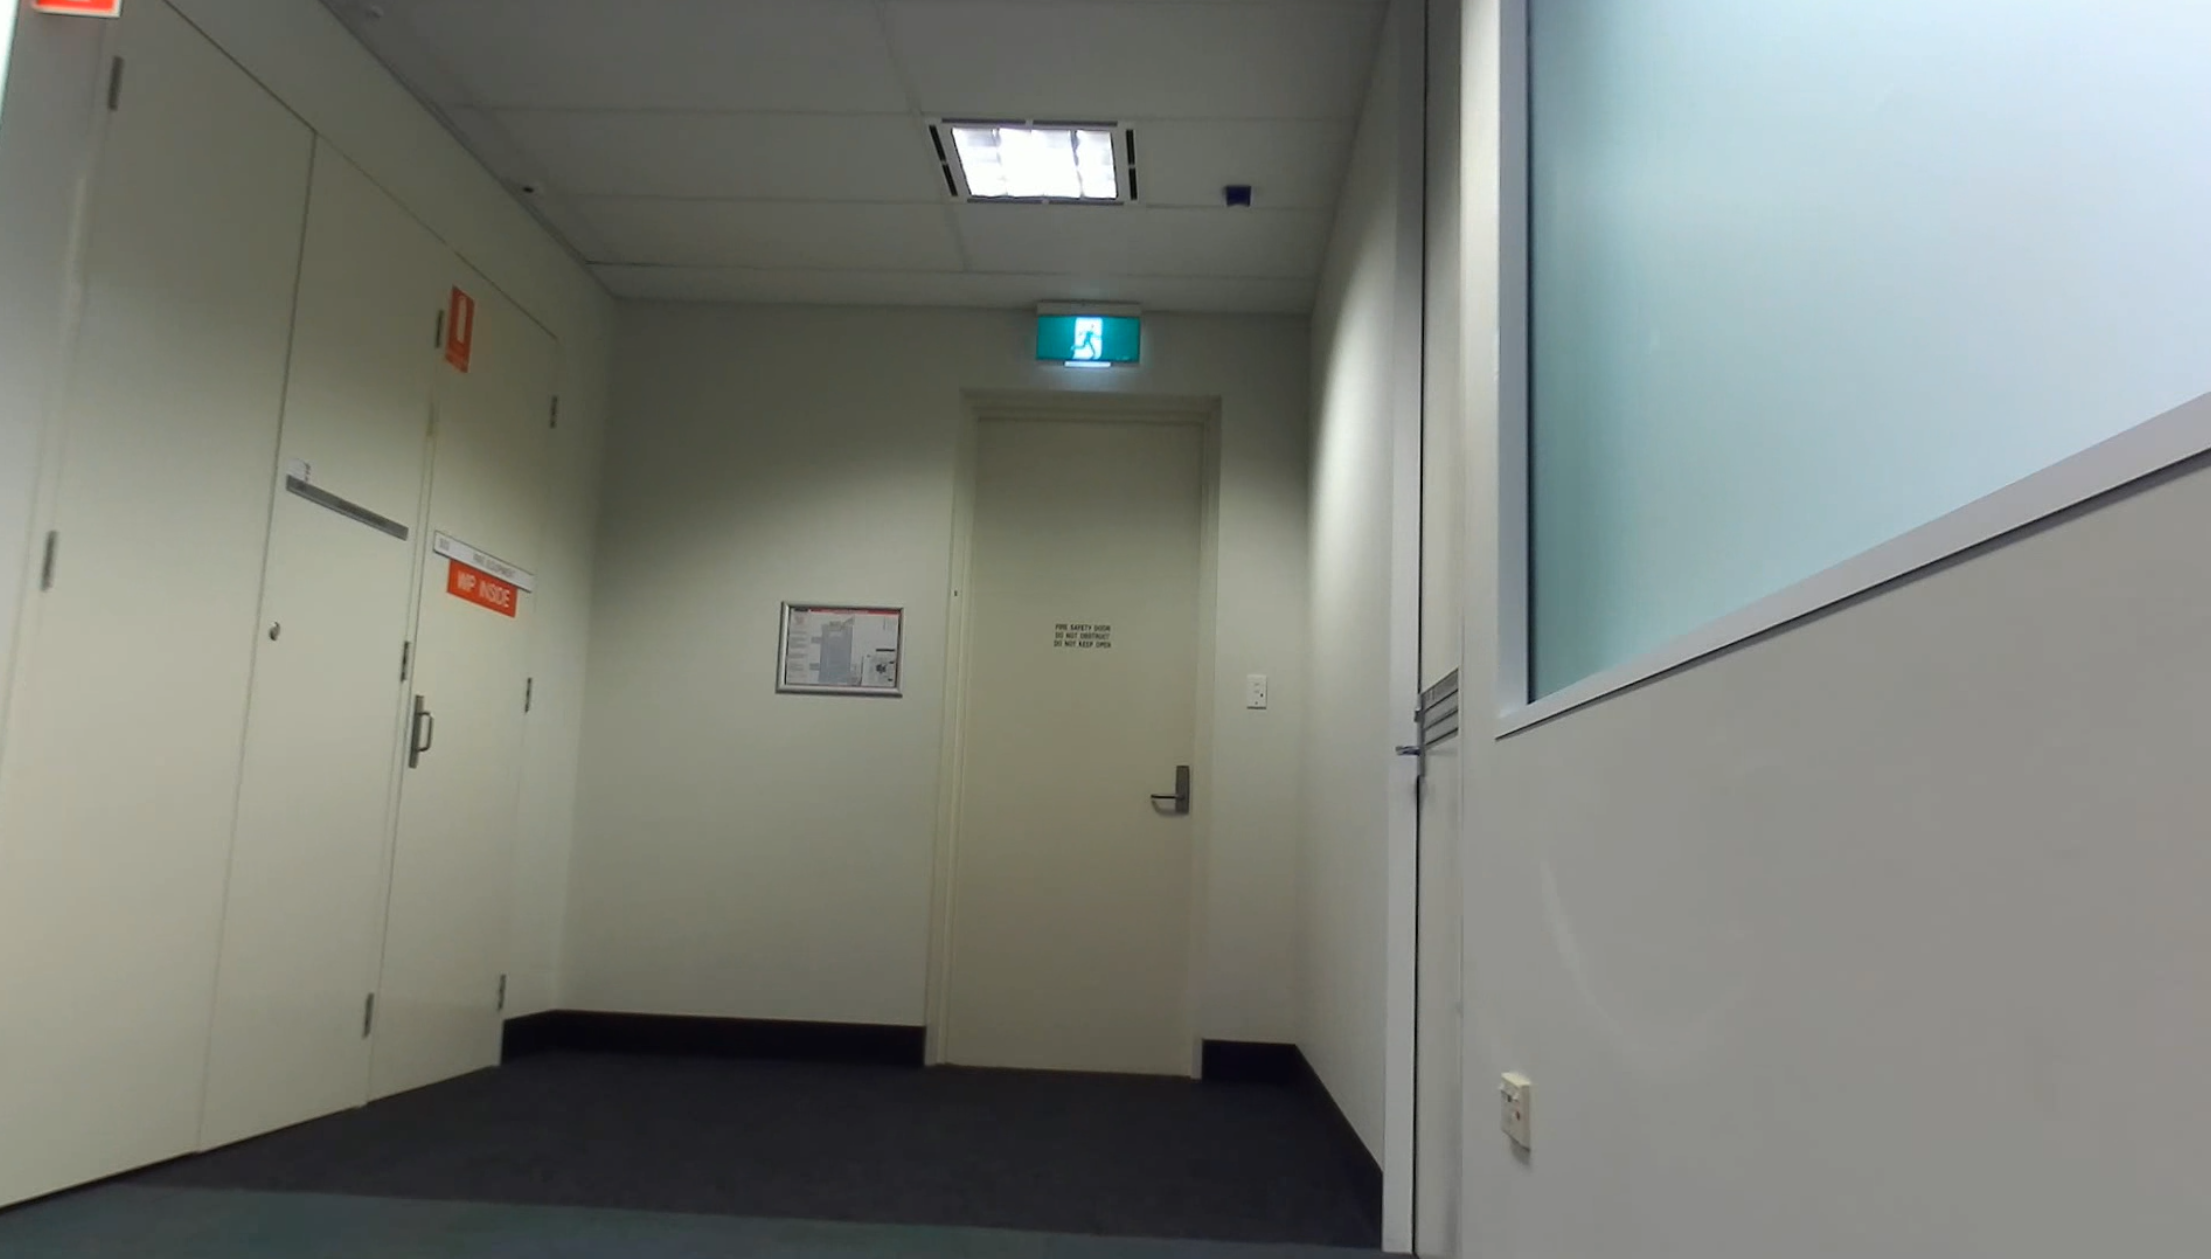
\includegraphics[width=\linewidth]{images/pcloud_indoor_comparison.PNG}
        \caption{Video footage}
    \end{subfigure}
    \begin{subfigure}{.2\textwidth}
        \centering
        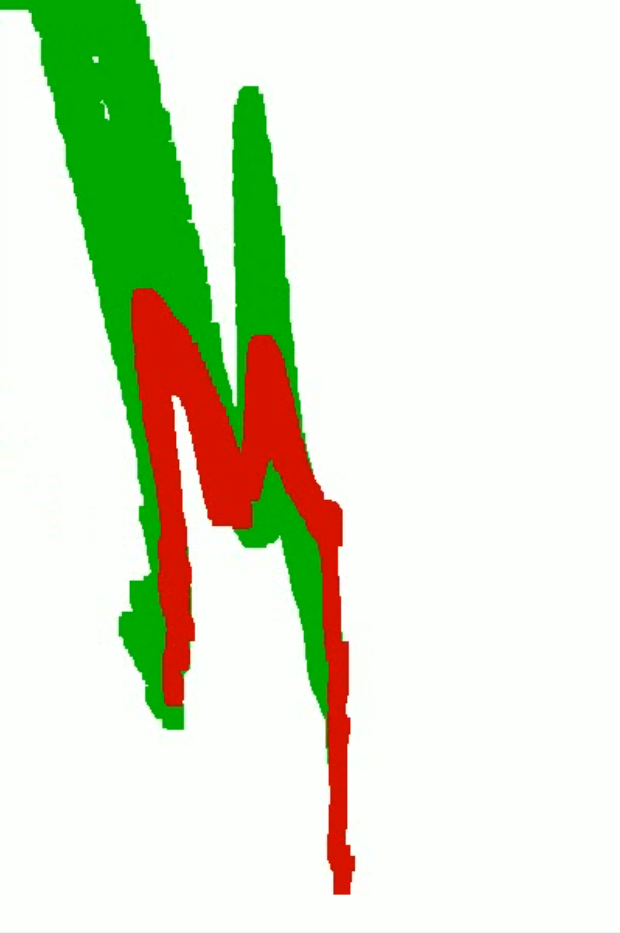
\includegraphics[width=\linewidth,frame]{images/pcloud_indoor_performance.PNG}
        \caption{Performance depth mode}
    \end{subfigure}
    \begin{subfigure}{.2\textwidth}
        \centering
        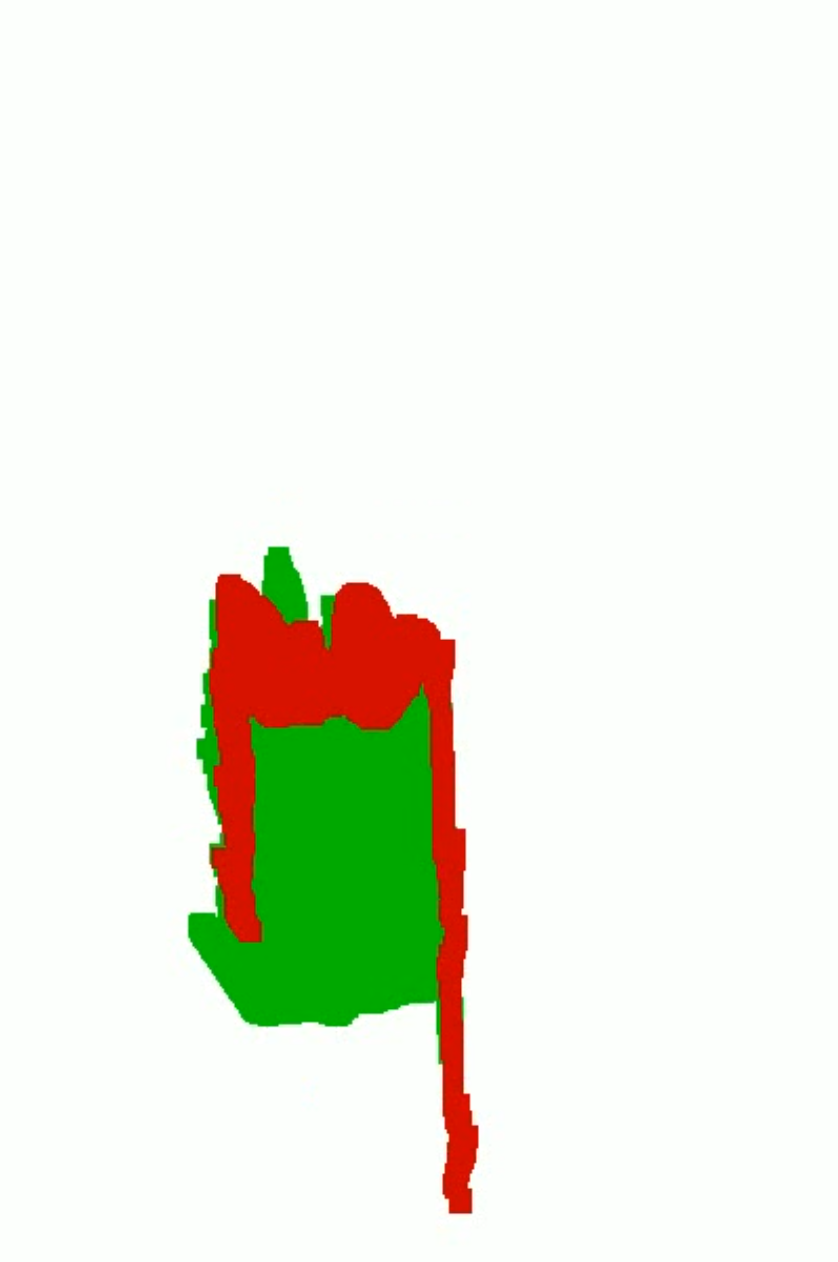
\includegraphics[width=\linewidth,frame]{images/pcloud_indoor_ultra.PNG}
        \caption{Ultra depth mode}
    \end{subfigure}
    \caption{Comparison of ZED Mini depth modes}
    \label{fig:depth_mode_comparison}
\end{figure}\clearpage

The ZED Mini has three depth modes: \texttt{ULTRA}, \texttt{QUALITY}, and \texttt{PERFORMANCE}.
These depth modes trade performance for depth accuracy - a comparison between the occupancy maps
generated by these modes can be seen in \cref{fig:depth_mode_comparison}.
The \texttt{ULTRA} depth mode accurately identifies the back wall as flat.
However, the \texttt{PERFORMANCE} depth mode does not identify the back wall
as flat, and incorrectly classifies an area beyond the wall as drivable.
Due to the high latency of the rest of this algorithm, the difference in speed between these two depth modes is negligible,
and therefore the \texttt{ULTRA} depth mode was selected.

%% can include some ramp comparisons if need be, but probably not

\subsection{Evaluation of assistive control algorithm}
VFH+ was implemented as a proof-of-concept assistive control algorithm.
This algorithm blends the user's target direction with the occupancy map
to determine a safe steering direction.

\Cref{fig:vfh_implementation} shows the VFH+ algorithm detecting an obstacle in front of
the wheelchair and steering left to avoid this obstacle. This
%demonstrates that  VFH+ works reliably as an assistive control algorithm and
showcases the end-to-end navigation assistance pipeline,
from environmental obstacle detection to
avoidance of that obstacle using VFH+.

The VFH+ algorithm takes
\SI{240}{\milli\second} to determine the steering direction, which increases to
\SI{430}{\milli\second} when called from Python due to the overhead of the MATLAB Engine API.
This latency could be a concern for a complete semi-autonomous wheelchair implementation;
however, this algorithm is a proof of concept, and latency was not a concern during implementation.
Additionally, VFH+ only adjusts the direction of the wheelchair and not the wheelchair's speed,
making it unsuitable as a final assistive control algorithm.

Due to the FOV of the camera, obstacles directly to the left or right of the wheelchair are not added
to the occupancy map. \Cref{fig:vfh_mistake} demonstrates a scenario where this can
become an issue. VFH+ mistakenly steers to the left to avoid the narrow hallway walls,
which would cause a crash with the walls directly to the left of the wheelchair.
This occurs because these walls are not in the occupancy map, and so the VFH+ algorithm
assumes that there is free space in this area.
Several approaches that could improve the occupancy map and rectify this issue
are suggested in \cref{sec:future_work}.

\setlength{\abovecaptionskip}{4pt}
\begin{figure}[p]
    % 16:6 width ratio
    % 0.64, 0.24
    \centering
    \begin{subfigure}{.5\textwidth}
        \centering
        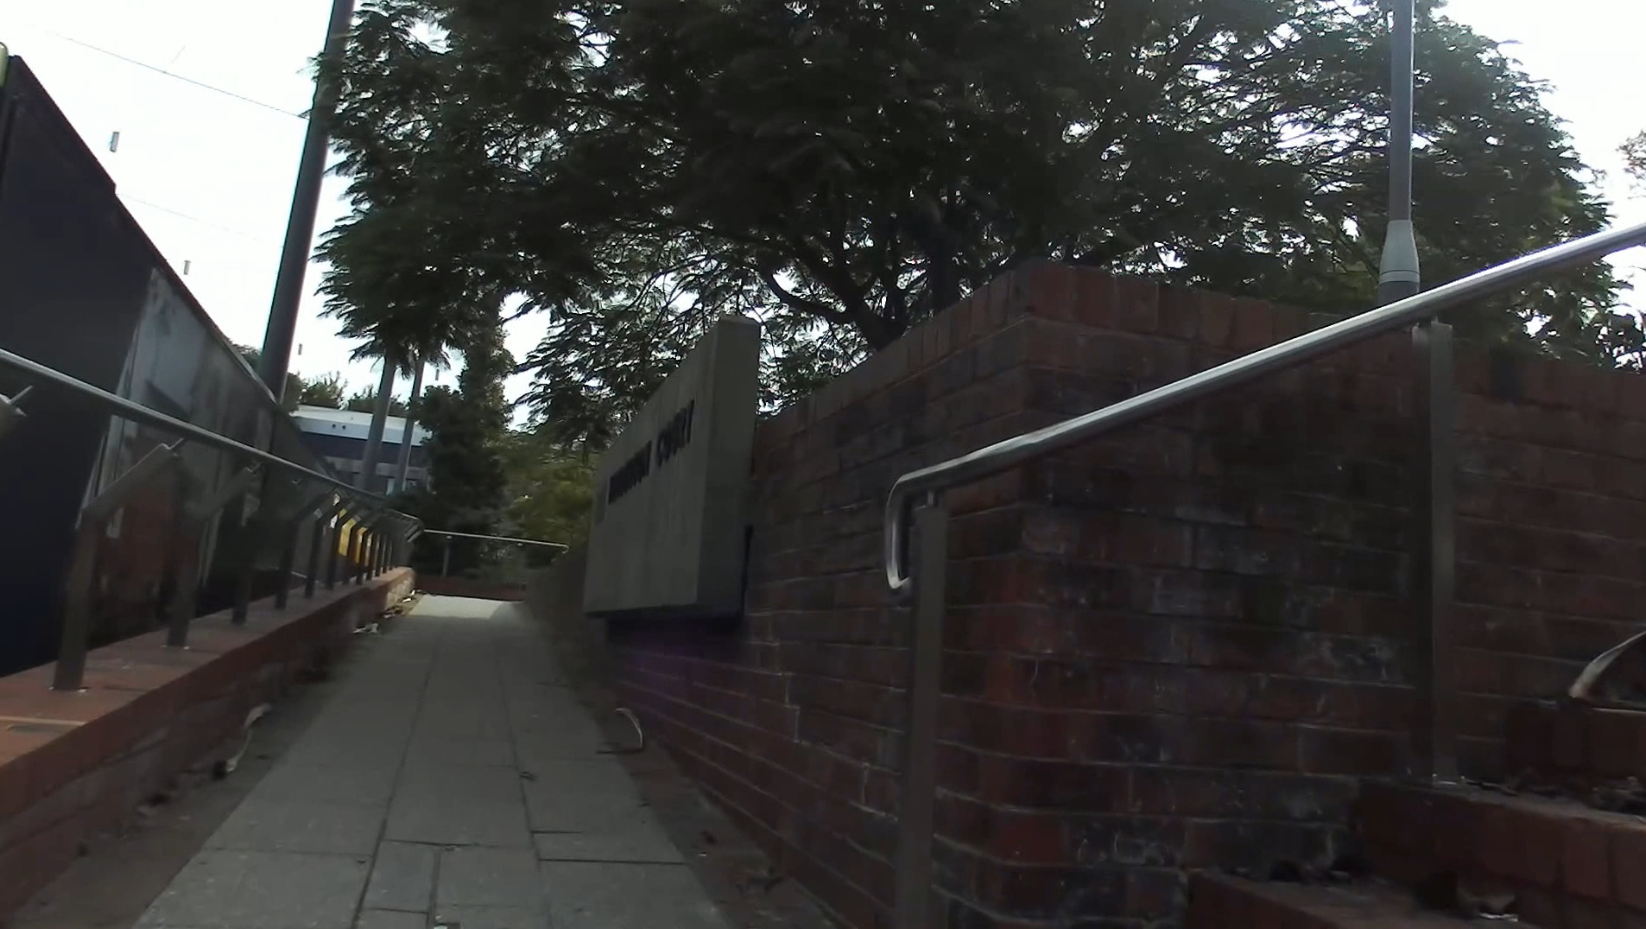
\includegraphics[width=\linewidth]{images/vfh_example_video.PNG}
        \caption{Video footage}
    \end{subfigure}
    \quad
    \begin{subfigure}{.2\textwidth}
        \centering
        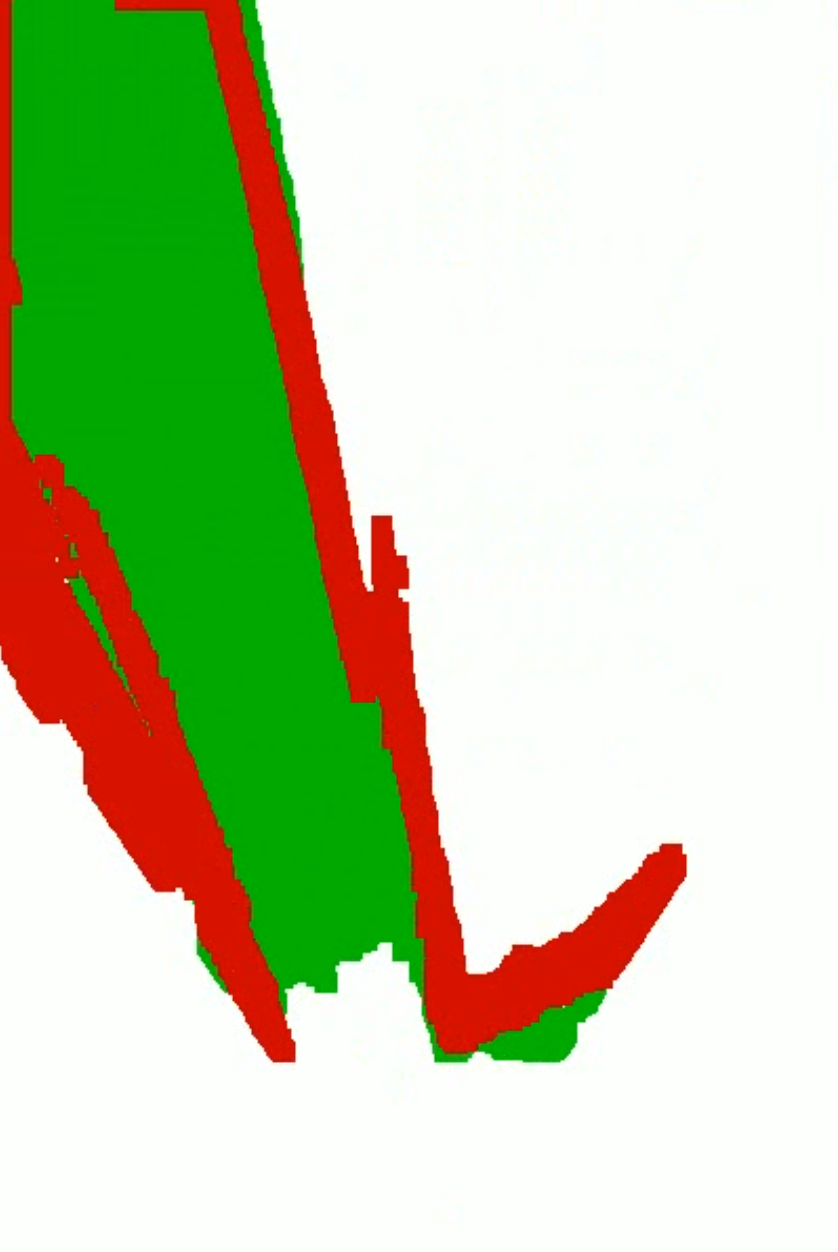
\includegraphics[width=\linewidth,frame]{images/vfh_example_map.PNG}
        \caption{Occupancy map}
    \end{subfigure}
    \begin{subfigure}{.4\textwidth}
        \centering
        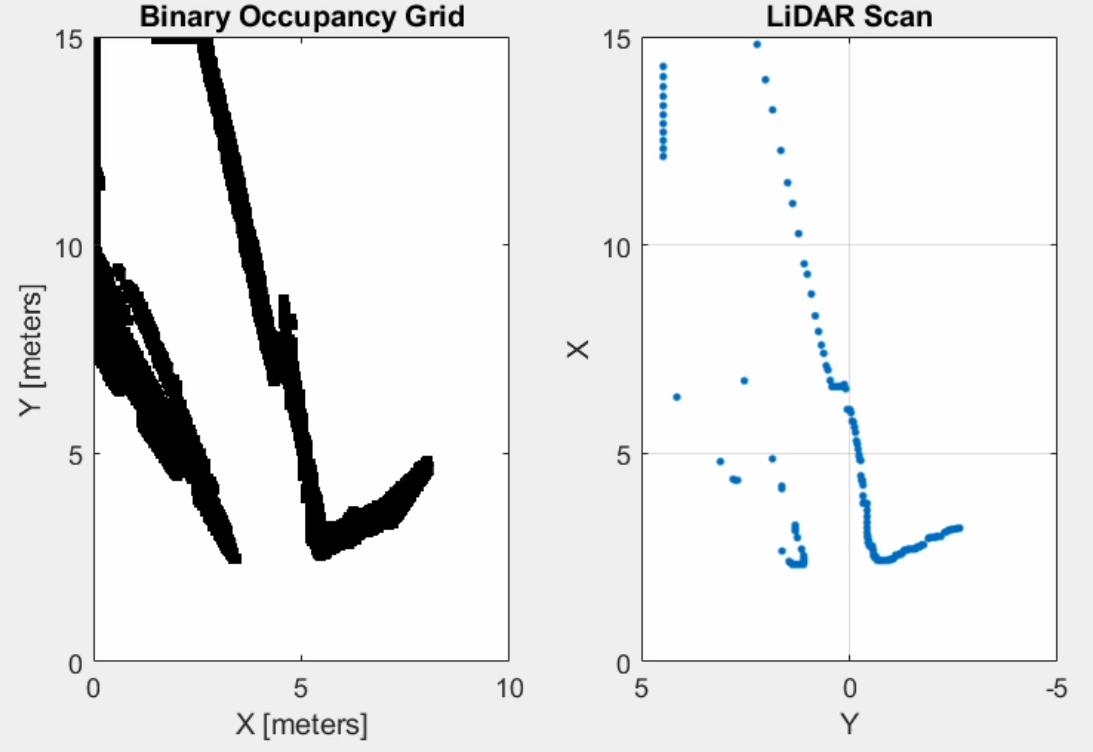
\includegraphics[width=\linewidth]{images/vfh_example_lidar.PNG}
        \caption{Binary occupancy grid and LIDAR scan of obstacles}
    \end{subfigure}
    \quad
    \begin{subfigure}{.55\textwidth}
        \centering
        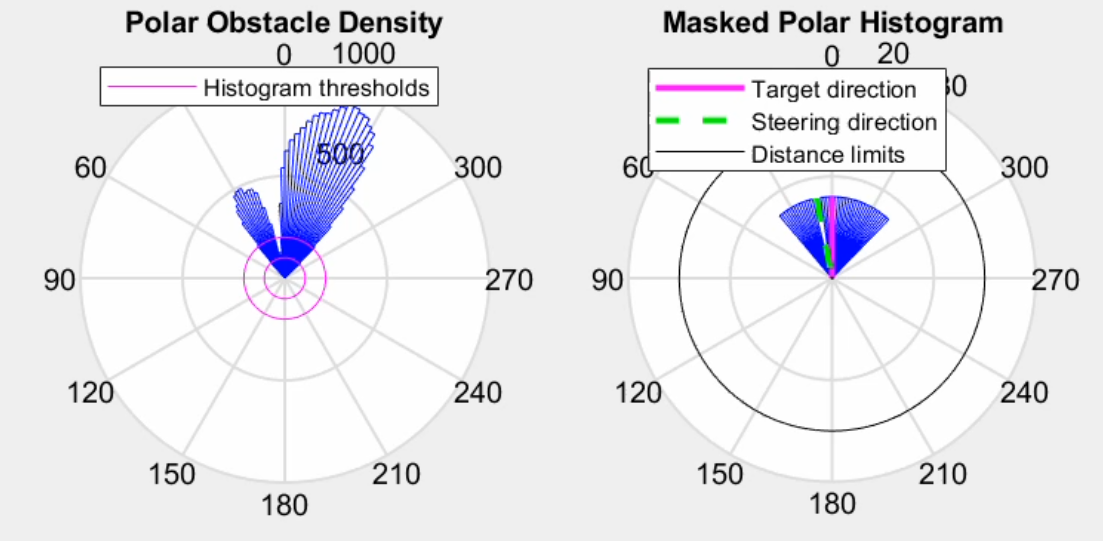
\includegraphics[width=\linewidth]{images/vfh_example_hist.PNG}
        \caption{Polar histogram of obstacles with target and steering directions}
    \end{subfigure}
    \caption{VFH+ changing direction to avoid an obstacle}
    \label{fig:vfh_implementation}
\end{figure}

\begin{figure}[p]
    % 16:6 width ratio
    % 0.64, 0.24
    \centering
    \begin{subfigure}{.5\textwidth}
        \centering
        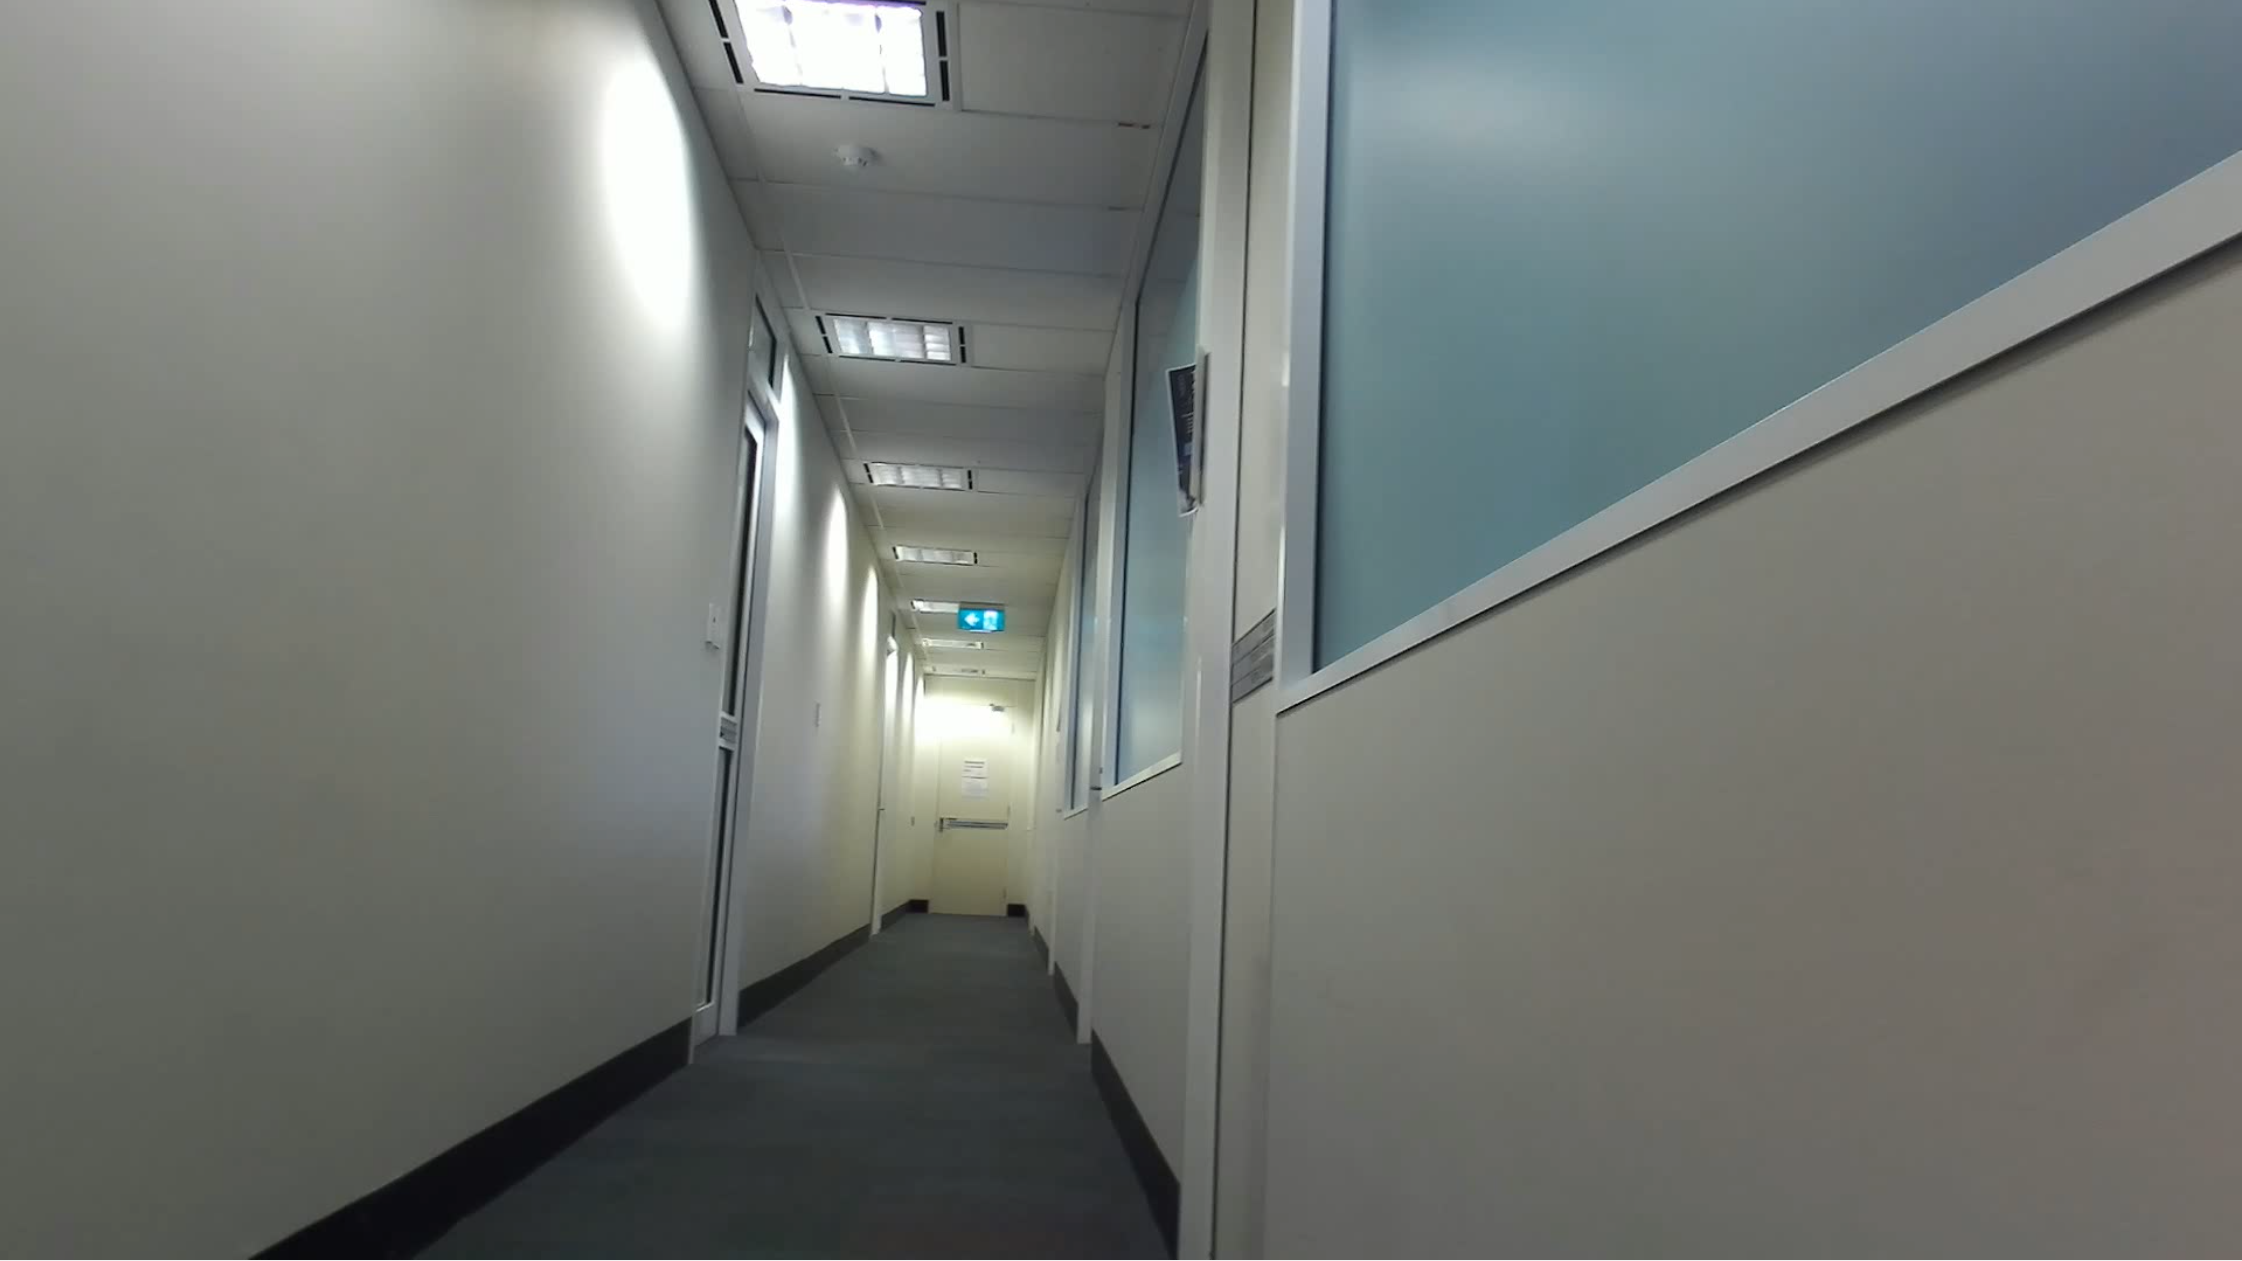
\includegraphics[width=\linewidth]{images/vfh_fov_video.PNG}
        \caption{Video footage}
    \end{subfigure}
    \quad
    \begin{subfigure}{.2\textwidth}
        \centering
        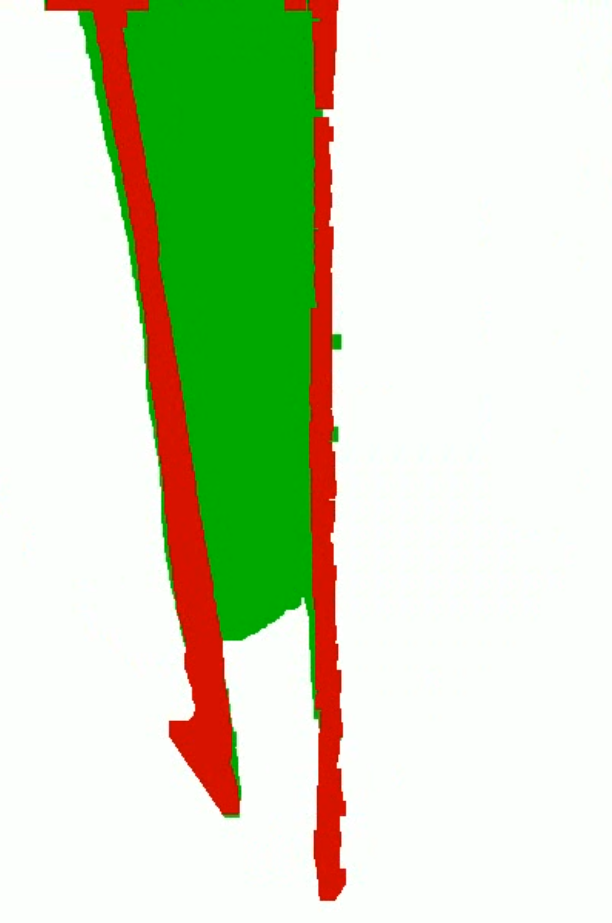
\includegraphics[width=\linewidth,frame]{images/vfh_fov_map.PNG}
        \caption{Occupancy map}
    \end{subfigure}
    \begin{subfigure}{.4\textwidth}
        \centering
        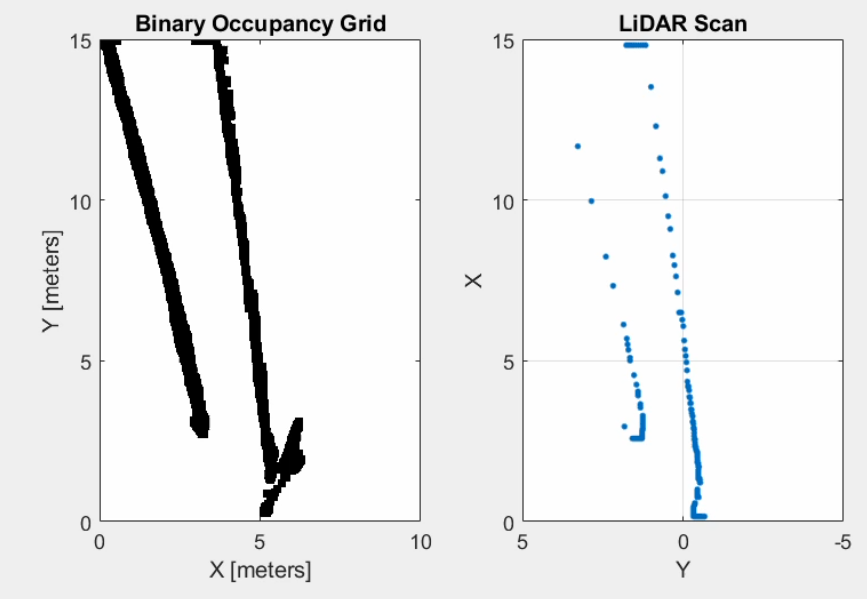
\includegraphics[width=\linewidth]{images/vfh_fov_lidar.PNG}
        \caption{Binary occupancy grid}
    \end{subfigure}
    \quad
    \begin{subfigure}{.55\textwidth}
        \centering
        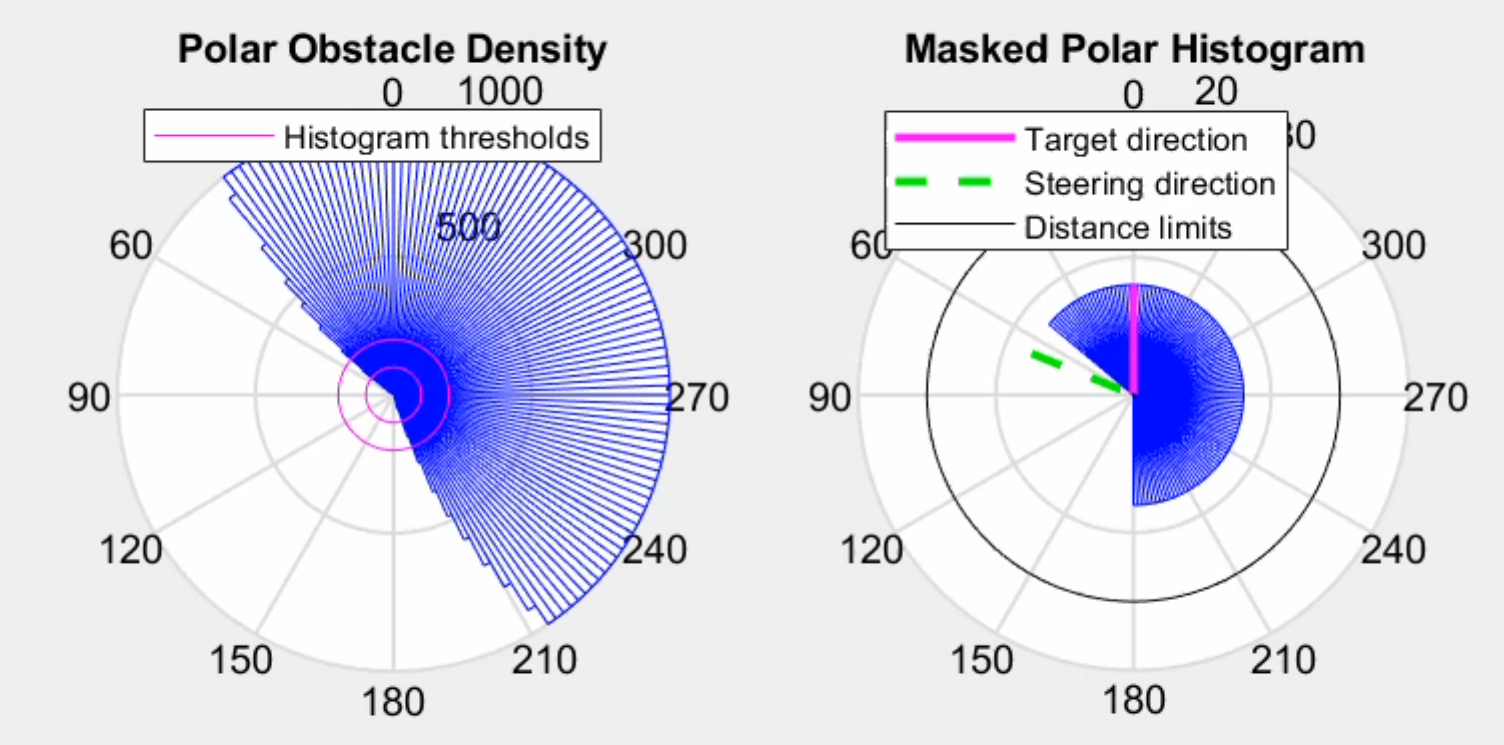
\includegraphics[width=\linewidth]{images/vfh_fov_hist.PNG}
        \caption{Polar histogram of obstacles}
    \end{subfigure}
    \caption{VFH+ mistakenly changing direction due to low sensor FOV}
    \label{fig:vfh_mistake}
\end{figure}\clearpage
\setlength{\abovecaptionskip}{12pt}

% include speed, turning behind
\subsection{Evaluation of pose estimation APIs}
The ZED Sensors API and ZED Positional Tracking API
were tested to estimate the pose of the wheelchair.

The Sensors API was able to produce accurate estimates
of the Euler angles of the ZED Mini. The camera has
a slight tilt which was noted in the dataset collection methodology
and measured as approximately 8.2\degree{} using point cloud data.
The IMU measures this tilt (x-axis rotation) to be approximately 8.5\degree{}
when travelling across flat ground, which agrees with the
point cloud tilt measurement to within 0.3\degree{}.

The Sensors API performs much worse when measuring the overall distance
travelled by the wheelchair. As part of the dataset, the wheelchair was
driven along the length of the Curtin bus station in a straight line,
for a distance of approximately \SI{83}{\metre} (measured using Google Maps).
The Sensors API is barely able to register any movement in the
wheelchair and records a distance of \SI{7.0}{\metre} in this time.

This error could be due to several factors. IMUs can have
high position errors (drift) as the position is calculated
by integrating the acceleration twice.
Additionally, the sampling rate of the sensors is \SI{800}{\hertz},
however is recorded in the dataset at \SI{30}{\hertz}. The lower
sampling rate could have helped these errors to propagate.
In this scenario, the wheelchair was travelling at a relatively constant
velocity, which would have caused the average acceleration to be close to zero throughout
the trip. A small error in the initial velocity estimate would have led to a larger
error in the resulting position estimate.

The Positional Tracking API, which combines sensor data with visual odometry,
was also tested in this scenario. This API recorded
a distance of \SI{127}{\metre}, which is larger
than the measured distance of \SI{83}{\metre} by 53\%.
The wheelchair's movement is plotted in \cref{fig:map_outline} and scaled to
show the actual path around the bus station; although the distance is not accurate,
the estimated path taken by the wheelchair is relatively accurate. Note that the measured distance only
consists of the path taken on the eastern side of the bus station.

A `jump' can be seen in \cref{fig:map_outline}; this can occur during visual odometry when
the positional tracking algorithm attempts to correct the ZED Mini's location. The Positional
Tracking API implements a parameter \texttt{enable\_pose\_smoothing} which is meant
to smooth the impact of this jump over several frames. However, some testing
indicates this feature is defective, as it produces completely unusable results
when used alongside \texttt{enable\_imu\_fusion} in ZED SDK version 3.7.7.

\begin{figure}[b]
    \centering
    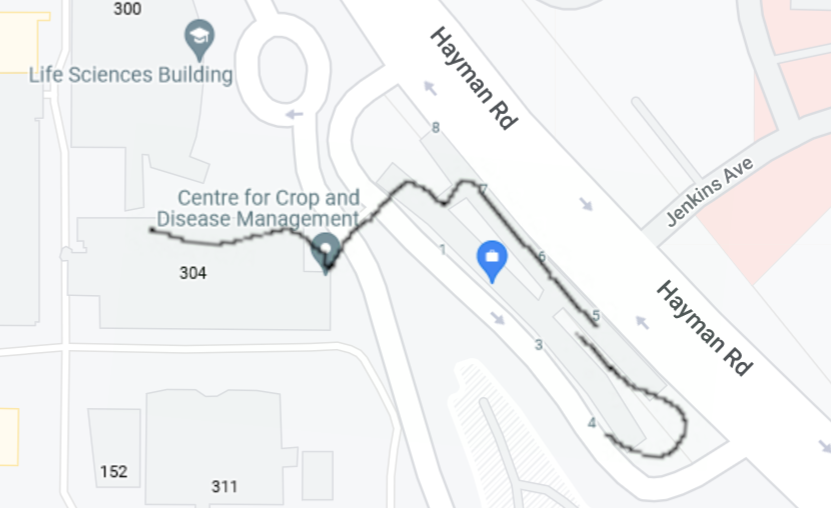
\includegraphics[width=0.7\linewidth,frame]{images/map_outline.png}
    \caption{Movement of the wheelchair around the Curtin bus station, recorded using the Positional Tracking API. Map data: Google \copyright 2022 \cite{googleGoogleMaps2022}}
    \label{fig:map_outline}
\end{figure}
